% This is samplepaper.tex, a sample chapter demonstrating the
% LLNCS macro package for Springer Computer Science proceedings;
% Version 2.20 of 2017/10/04
%
\documentclass[runningheads]{llncs}
%
\usepackage[T1]{fontenc}
\usepackage{multirow}
\usepackage{graphicx}
\usepackage{textcomp}
%\usepackage[firstpage]{draftwatermark}

%\SetWatermarkColor[gray]{0.95}
%\SetWatermarkText{Review}
%\SetWatermarkScale{5}
\usepackage[export]{adjustbox}
%\usepackage{setspace}
% Used for displaying a sample figure. If possible, figure files should
% be included in EPS format.
%
% If you use the hyperref package, please uncomment the following line
% to display URLs in blue roman font according to Springer's eBook style:
% \renewcommand\UrlFont{\color{blue}\rmfamily}

% Added by Dhaminda
%\setlength{\belowcaptionskip}{-20pt}

\usepackage{todonotes}

%\usepackage[
%backend=biber,
%style=numeric-comp,
%maxcitenames=1,
%maxbibnames=2,
%backref=true
%]{biblatex}

\hyphenation{pro-ba-bi-lis-tic}

\begin{document}
	%
	\title{AERoS: Assurance of Emergent Behaviour in Autonomous Robotic Swarms}%\thanks{\dag D. B. Abeywickrama and J. Wilson contributed equally.}}
%
\titlerunning{AERoS: Assurance of Emergent Behaviour in Autonomous Robotic Swarms}%{Abbreviated paper title}
% If the paper title is too long for the running head, you can set
% an abbreviated paper title here
%
%\author{Dhaminda B. Abeywickrama\inst{\dag}\inst{1}\orcidID{0000-0002-4423-0284} \and \\
%	James Wilson\inst{\dag}\inst{1}\orcidID{0000-0002-0758-6732} \and
%	Suet Lee\inst{1}\orcidID{0000-0002-9196-5769} \and \\
%	Greg Chance\inst{1}\orcidID{0000-0001-5334-370X} \and
%	Peter D. Winter\inst{1}\orcidID{0000-0003-0766-6297} \and
%	Arianna Manzini\inst{1}\orcidID{0000-0001-7710-8974} \and 
%	Ibrahim Habli\inst{2}\orcidID{0000-0003-2736-8238} \and 
%	Shane Windsor\inst{1}\orcidID{0000-0002-7597-4497} \and
%	Sabine Hauert\inst{1}\orcidID{0000-0003-0341-7306} \and
%	Kerstin Eder\inst{1}\orcidID{0000-0001-9746-1409}}
\author{Dhaminda B. Abeywickrama\inst{\dag}\inst{1} \and 
	James Wilson\inst{\dag}\inst{1} \and
	Suet Lee\inst{1} \and \\
	Greg Chance\inst{1} \and
	Peter D. Winter\inst{1} \and
	Arianna Manzini\inst{1} \and 
	Ibrahim Habli\inst{2} \and  \\
	Shane Windsor\inst{1} \and
	Sabine Hauert\inst{1} \and
	Kerstin Eder\inst{1}}

\authorrunning{D.B.\ Abeywickrama and J.\ Wilson et al.}

\institute{University of Bristol, Bristol, UK \\
	\email{\{firstname.lastname\}@bristol.ac.uk} \and
	University of York, York, UK\\
	\email{ibrahim.habli@york.ac.uk}}

%\institute{Princeton University, Princeton NJ 08544, USA \and
%	Springer Heidelberg, Tiergartenstr. 17, 69121 Heidelberg, Germany
%	\email{lncs@springer.com}\\
%	\url{http://www.springer.com/gp/computer-science/lncs} \and
%	ABC Institute, Rupert-Karls-University Heidelberg, Heidelberg, Germany\\
%	\email{\{abc,lncs\}@uni-heidelberg.de}}
%
%\institute{University of Bristol, Bristol, UK\\
%	\email{\{firstname.lastname\}@bristol.ac.uk}}
%\institute{University of York, York, UK\\
%	\email{\{ibrahim.habli\}@york.ac.uk}}
%%
\maketitle              % typeset the header of the contribution
%
\begin{abstract} 
%The overall behaviours of a swarm are not explicitly engineered in the system. However, they are an emergent consequence of the interaction of individual agents with each other and their environment. 
%This emergent functionality poses a challenge to ensure their \emph{assurance}, such as safety. 
%The main contribution of this paper is a process for the safety assurance of the emergent behaviour for use in autonomous robotic swarms called \emph{AERoS}, following the AMLAS guidance for machine learning systems. 
%We explore our proposed guidance using an illustrative case study centred on a robot swarm operating a public cloakroom.
% OLD> We explore our proposed guidance using illustrative examples taken from a public cloakroom case study.
The behaviours of a swarm are not explicitly engineered. Instead, they are an emergent consequence of the interactions of individual agents with each other and their environment.
This emergent functionality poses a challenge to \emph{safety assurance}. %, such as safety assurance.
The main contribution of this paper is a process for the safety assurance of emergent behaviour in autonomous robotic swarms called \emph{AERoS}, following the guidance on the Assurance of Machine Learning for use in Autonomous Systems (AMLAS). 
We explore our proposed process using a case study centred on a robot swarm operating a public cloakroom.
	
\keywords{Assurance \and Safety \and Emergent behaviour \and Guidance \and Swarms.}
\end{abstract}


\section{Introduction}\label{introduction}
%\todo{A friend of mine (who worked for an insurance company as safety inspector) read this and asked after the first page, whether this is grounded or airborne. This ought to be made clear at the start.}
% Dhaminda - this has been addressed. Please check. 
%\todo{SW: Please check referencing commands - not clear why first reference is 13}
%Dhaminda: We are using the bibliographystyle provided by the template without any changes. The template has been double checked and it is correct. \bibliographystyle{splncs04}
Swarm robotics provides an approach to the coordination of large numbers of robots inspired by swarm behaviours in nature. %~\cite{Sahin2005}. 
%The functionality of a swarm is emergent, and evolves based on the capabilities of the robots and the numbers of robots used. 
The overall behaviours of a swarm are not explicitly engineered in the system~\cite{Winfield2006,Abeywickrama2022}. 
Instead, they are an emergent consequence of the interactions of individual agents with each other and the environment, we call this emergent behaviour (EB)~\cite{Abeywickrama2022}. 
EB can be difficult to model and characterize and this property of swarms poses a critical challenge to \emph{assurance}~\cite{Cheng2014}. 
%; this poses a challenge to \emph{assurance}~\cite{Cheng2014}.
%Instead, they are an emergent consequence of the interactions of individual agents with each other and the environment; this poses a challenge to \emph{assurance}~\cite{Cheng2014}.
%The overall behaviours of a swarm are not explicitly engineered in the system. Instead, they are an emergent consequence of the interactions of individual agents with each other and the environment~\cite{Abeywickrama2022}; this poses a challenge to \emph{assurance}. 
%\emph{Assurance} is defined as ``all the planned and systematic activities implemented within the quality system, and demonstrated as needed, to provide adequate confidence that an entity will fulfil requirements for quality''~\cite{ISO24765:2017}. 
%According to the ISO standard for systems and software engineering vocabulary~\cite{ISO24765:2017}, \emph{assurance} is defined as ``all the planned and systematic activities implemented within the quality system, and demonstrated as needed, to provide adequate confidence that an entity will fulfil requirements for quality''. 
Assurance tasks comprise conformance to standards, verification and validation (V\&V), and certification. Assurance criteria for autonomous systems (AS) include both functional and non-functional requirements such as safety~\cite{Cheng2014}. 

Existing standards and regulations of AS are either implicitly or explicitly based on the V lifecycle model~\cite{Jia2021}. %, which moves from requirements through design onto implementation and testing before deployment~\cite{Jia2021}. 
%Existing standards and regulations of AS are either implicitly or explicitly based on the V-model~\cite{Forsberg:1992}, which moves from requirements through design onto implementation and testing before deployment~\cite{Jia2021,Fisher2020}. 
However, this model is unlikely to be suitable for systems with EB; for example\ through interaction with other agents and the environment, as is the case with swarms. 
ISO standards have been developed for the service robotics sector (non-industrial) (e.g.\ ISO 13482, ISO 23482-1), and the industrial robotics sector (e.g.\ ISO 10218-1, ISO/TS 15066)~\cite{Abeywickrama2022}. 
However, although these standards focus on ensuring the assurance of robots at the individual level, they do not cover safety at the \emph{swarm} level that may arise through EB. 
%There have been several standards and guidance introduced by various industry committees and research groups. 
%In 2016, the British Standards Institution introduced the BS 8611 standard that provides a guide to the ethical design and application of robots and robotic systems. % \cite{BS8611}. 
%Then, IEEE initiated the development of a series of standards to address autonomy, ethical issues, transparency, data privacy and trustworthiness (e.g. IEEE P7001, P7010).  
%
\subsubsection{Related Work} There are several standards and guidance related to machine learning (ML) in aeronautics, automotive, railway and industrial domains \cite{Kaakai2022}, for example the AMLAS process~\cite{Hawkins2021}, the European Union Aviation Safety Agency (EASA) concept paper, the DEpendable and Explainable Learning (DEEL) white paper, the Aerospace Vehicle System Institute (AVSI) report, the Laboratoire National de Métrologie et d'Essais (LNE) certification, and the UL 4600 standard. However, none of these approaches targets robot swarms. 
In this work we used AMLAS \cite{Hawkins2021} as the foundation for developing an assurance process for autonomous robotic swarms. 
AMLAS provides guidance on how to systematically integrate safety assurance into the development of the ML components based on offline supervised learning. 
AMLAS contains six stages where assurance activities are performed in parallel to the development activities. 
AMLAS has the advantage of ensuring safety assurance for complex AS where the behaviour of the system is controlled by ML algorithms. 
Our study takes inspiration from AMLAS, but adapt it to focus on emergence as the driver for complexity, rather than learning. 
%In this work, we take inspiration from AMLAS, but adapt it to focus on emergence as the driver for complexity, rather than learning. 
%However, although these standards focus on ensuring the assurance of robots at the individual level, they do not cover safety or any other extra-functional property at the \emph{swarm} level that may arise through EB. 
\vspace{-2ex}
\subsubsection{Main Contribution and Paper Outline} In this work, we propose a process for the safety assurance of EB in autonomous robotic swarms (AERoS), adapted from the guidance on the Assurance of Machine Learning for use in Autonomous Systems (AMLAS)~\cite{Hawkins2021}. 
AERoS covers six EB lifecycle stages: safety assurance scoping, safety requirements elicitation, data management, model EB, model verification, and  model deployment. 
The AERoS process is domain independent and therefore can be applied to any swarm type (e.g. grounded, airborne). 
%Also, a system of components can be considered as analogous to a swarm if the system is decentralized with local interactions between components. AERoS may be applicable in such cases as well. 
In particular, a system of components can be considered as analogous to a swarm if the system is decentralized with local interactions between components. 
AERoS may be applicable in such cases as well. % - in this case the AERoS process may also be applicable. 
In this paper, we explore the AERoS process using a case study centered on a robot swarm operating a public cloakroom at events with 50 to 10000 attendees~\cite{Jones2020}. 
In the cloakroom, a swarm of robots assist attendees to deposit, store, and deliver their belongings (e.g. jackets) \cite{Jones2020}. 
As the swarm operates in a public setting, the system must prioritise public safety (e.g. avoid harm from collisions, fire hazards caused by blockages). 
The rest of the paper is organised as follows. 
%In Section~\ref{relatedwork}, we provide key related work to our study. 
%Section~\ref{framework} discusses the six stages of AERoS, and in Section~\ref{discussion-conclusions} we provide a brief discussion and concludes the paper.
In Section~\ref{framework}, we discuss the six stages of AERoS. Section~\ref{discussion-conclusions} provides a brief discussion and concludes the paper. 

%\section{Related Work}\label{relatedwork}
%There are several standards and guidance related to machine learning in aeronautics, automotive, railway and industrial domains \cite{Kaakai2022}, for example the AMLAS process~\cite{Hawkins2021}, the European Union Aviation Safety Agency (EASA) concept paper, the DEpendable and Explainable Learning (DEEL) white paper, the Aerospace Vehicle System Institute (AVSI) report, the Laboratoire National de Métrologie et d'Essais (LNE) certification, and the UL 4600 standard. However, none of these approaches targets robot swarms. 
%In this work we used AMLAS \cite{Hawkins2021} as the foundation for developing an assurance process for autonomous robotic swarms. 
%AMLAS provides guidance on how to systematically integrate safety assurance into the development of the machine learning components based on offline supervised learning. 
%AMLAS contains six stages where assurance activities are performed in parallel to the development activities. 
%AMLAS has the advantage of ensuring safety assurance for complex AS where the behaviour of the system is controlled by machine learning algorithms. 
%In this work, we take inspiration from AMLAS, but adapt it to focus on emergence as the driver for complexity, rather than learning. 

\section{The AERoS Process}\label{framework}
This section discusses the six main stages of AERoS targeting autonomous robot swarms. AERoS is iterative by design, and the assurance activities are performed in parallel to EB development (see Fig.~\ref{aeros-process}). For each stage, we describe its inputs and outputs, main assurance activities and their associated artefacts. 
%In this section, we discuss the six main stages of the AERoS process targeting autonomous robot swarms. For each stage, we describe its inputs and outputs, main assurance activities and their associated artefacts. AERoS is iterative by design, and the assurance activities are performed in parallel to the development activities (see Fig.~\ref{aeros-process}).
%AERoS is iterative by design, and contains six stages where assurance activities are performed in parallel to the development activities. 
\begin{figure*}[!t]
	\centering
	\vspace{-2ex}
	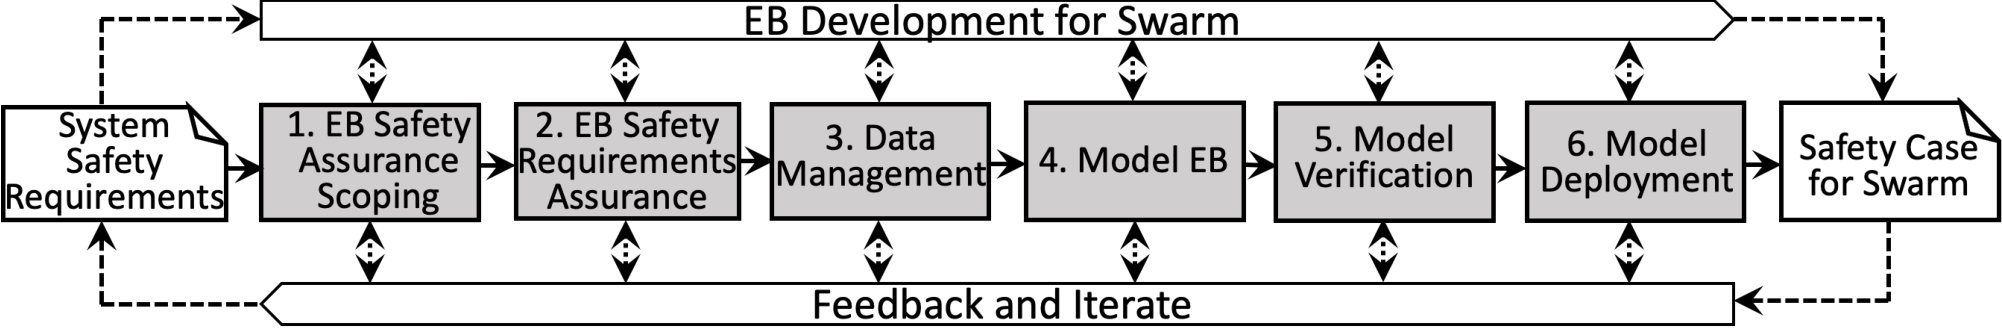
\includegraphics[width=0.95\textwidth]{figures/AERoS-Process.pdf}%AMLAS-STAGE-3-V4.png
	\vspace{-3ex}
	\caption{The AERoS process with the six stages adapted from AMLAS.}%: iterative-by-design and the six stages where assurance activities are performed in parallel to development. 
	\label{aeros-process}
	\vspace{-3ex}
\end{figure*}
%\begin{figure*}[!b]
%	\centering
%	\vspace{-4ex}
%	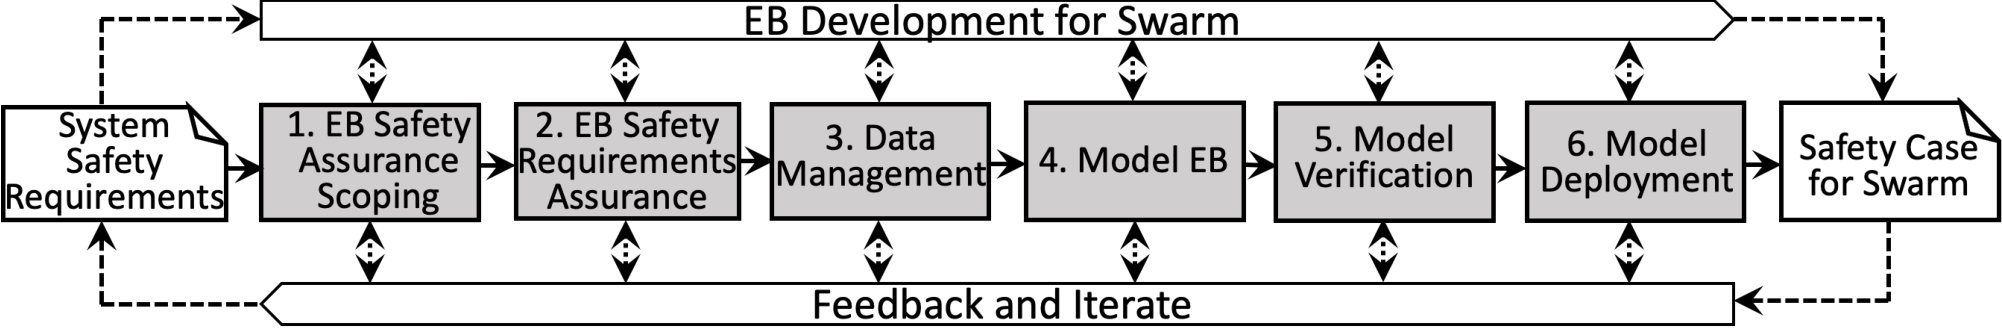
\includegraphics[width=0.95\textwidth]{figures/AERoS-Process.pdf}%AMLAS-STAGE-3-V4.png
%	\vspace{-3ex}
%	\caption{The AERoS process with the six stages adapted from AMLAS.}%: iterative-by-design and the six stages where assurance activities are performed in parallel to development. 
%	\label{aeros-process}
%	\vspace{-4ex}
%\end{figure*}
%In this study, we look at inherent swarm qualities and the adaptation that arises from these qualities. 
%In a swarm, individual robots execute simple behaviours or algorithms, and these simple behaviours when performed by a large number of agents build to form \emph{emergent behaviours} (EB).  
%
%We will consider the adaptation of individual agents using machine learning in future work. 
%At present, our study does not consider machine learning components of individual agents. 
%The adaptivity provided by this emergence requires us to provide \emph{assurance} (e.g. safety assurance). 
%In this study, we investigate inherent swarm qualities and the adaptation that arises from these qualities. 
%%%%These simple behaviours performed by large numbers of agents build to emergent behaviours.
%%%%For this, we will look into developing individual behaviours which when combined create an adaptive emergence. 
%The adaptivity provided by this emergence requires us to provide \emph{assurance} (e.g. safety assurance). 
%At present, our study does not consider machine learning components of individual agents. 
%Instead, these will be considered as part of future work once AMLAS has been applied to the swarm.
%However, we may consider this later once AMLAS has been applied to the swarm.

\subsection{Stage 1: EB Safety Assurance Scoping} \label{framework-stage1}
Stage 1 contains two activities which are performed to define the safety assurance scope for the swarm (see Fig.~\ref{amlas-a-stage1}). 
%In a swarm, individual robots execute simple behaviours, and when performed by a large number of agents, these simple behaviours build to form EB.

\noindent\textbf{Activity 1. Define Assurance Scope for the EB Description and Expected Output}
%The goal of Activity 1, which has four inputs [A--D] (Fig.~\ref{amlas-a-stage1}), is to define the safety assurance scope for the EB and expected output. 
The goal of Activity 1 (Fig.~\ref{amlas-a-stage1}) is to define the safety assurance scope for the EB and expected output. 
%The output of this activity is the Safety Requirements Allocated to the Swarm [E]. 
The requirements defined in this stage are independent of any EB technology, which reflects the need for the robot swarm to perform safely regardless of emergence. 

\emph{[A] System Safety Requirements:}
The system safety assessment process generates the safety requirements of the swarm, and covers the identification of hazards (e.g. the blocking of critical paths in the cloakroom) and risk analysis.
Figure~\ref{failure-events} illustrates how individual robot failures propagate through the neighbourhood to swarm-level hazards: we can then derive safety requirements in the form of concrete failure conditions at the level of the whole swarm which capture, implicitly, all levels of the swarm. 
%Although this has been illustrated as a simplified linear chain of events, in reality this represents a complex sequence which can be difficult to distil into distinct events and causes. 

\emph{[B] Environment Description:}
It is essential to consider the system environment when allocating safety requirements to the swarm. 
In the cloakroom, a swarm of robotic agents collects and delivers jackets, which are stored in small box-like containers. 
The agents are required to navigate a public space between collection and delivery points. 
%They use local communication, perception, and data to form an emergent system of navigation which allows them to easily traverse the public space. 
%Dhaminda Slightly increased size of Fig. 1 16/02/23
\begin{figure}[!b]
	\vspace{-6ex}
	\centering
	\begin{minipage}[b]{.5\textwidth}
		\centering
		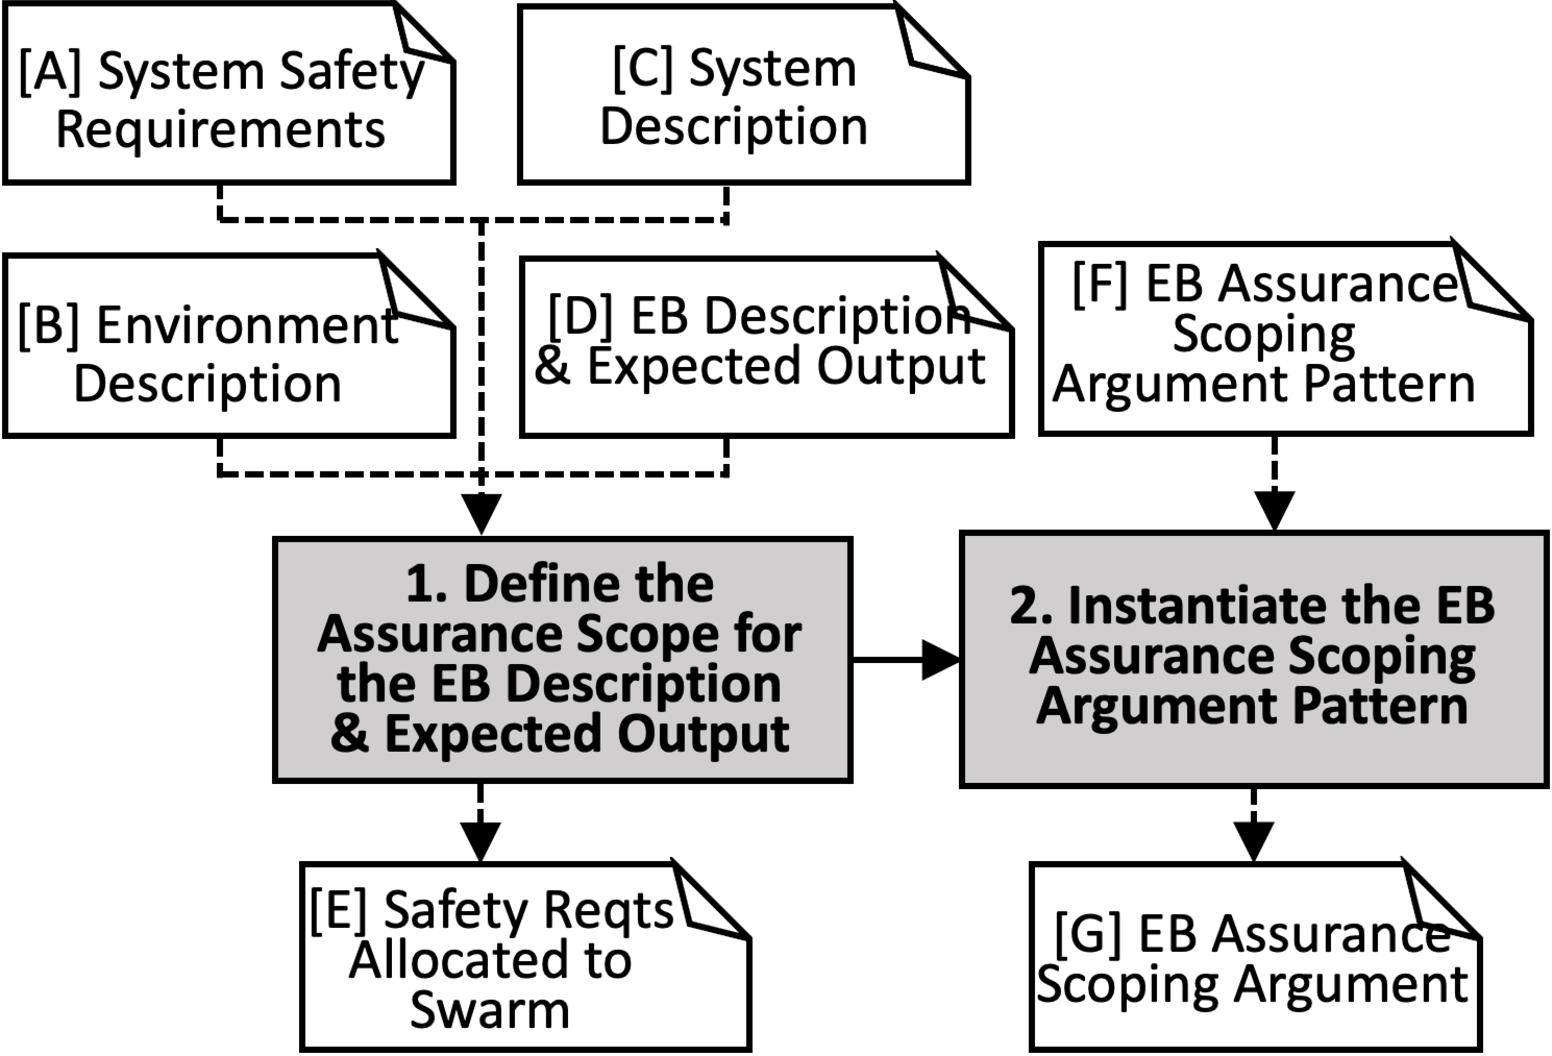
\includegraphics[width=0.99\textwidth]{figures/AERoS-Stage1.pdf}%AERoS-Stage1-v3.png AERoS-Stage1-v2.png
		\vspace{-1ex}%-2ex
		\caption{Stage 1: The AERoS emergent behaviour assurance scoping process.}
		\label{amlas-a-stage1}
	\end{minipage}%
	\hspace*{.03\textwidth}
	\begin{minipage}[b]{.5\textwidth}
		%\centering
		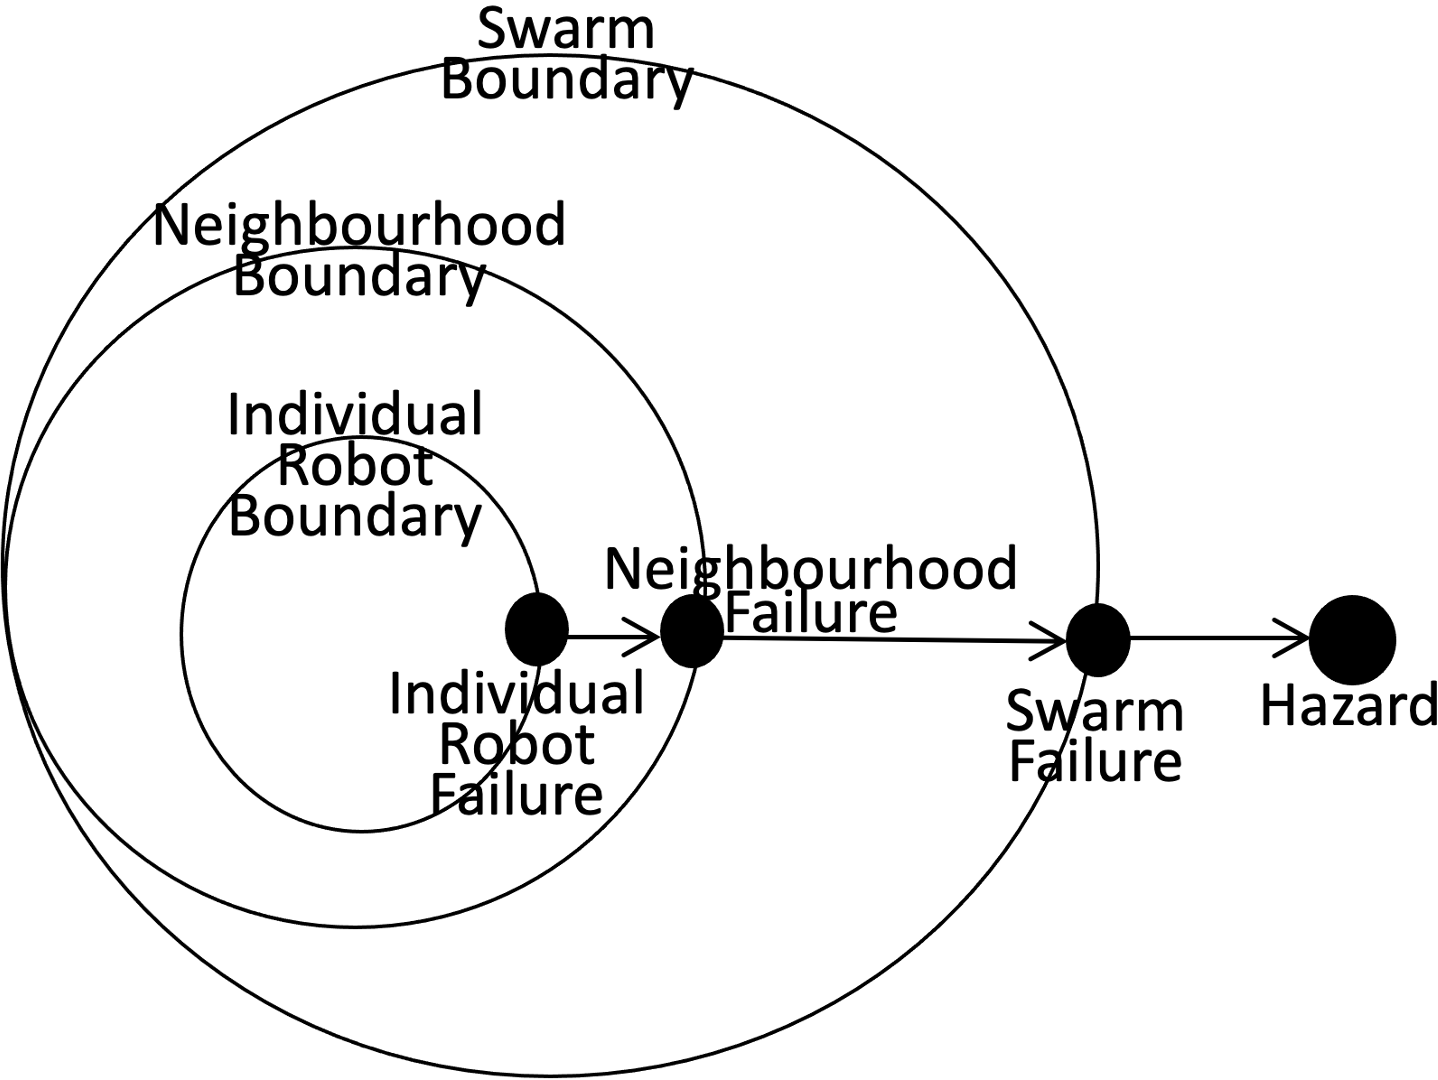
\includegraphics[width=0.99\textwidth]{figures/stage1-failureevents-v4.png}
		\vspace{-4ex}%-2ex
		\caption{Failure conditions in a swarm adapted from DO-178C and AMLAS.}
		\label{failure-events}
	\end{minipage}
	\vspace{-7ex} % 4ex
\end{figure}
%\begin{figure}[!t]
%	\centering
%	\begin{minipage}[b]{.5\textwidth}
%		\centering
%		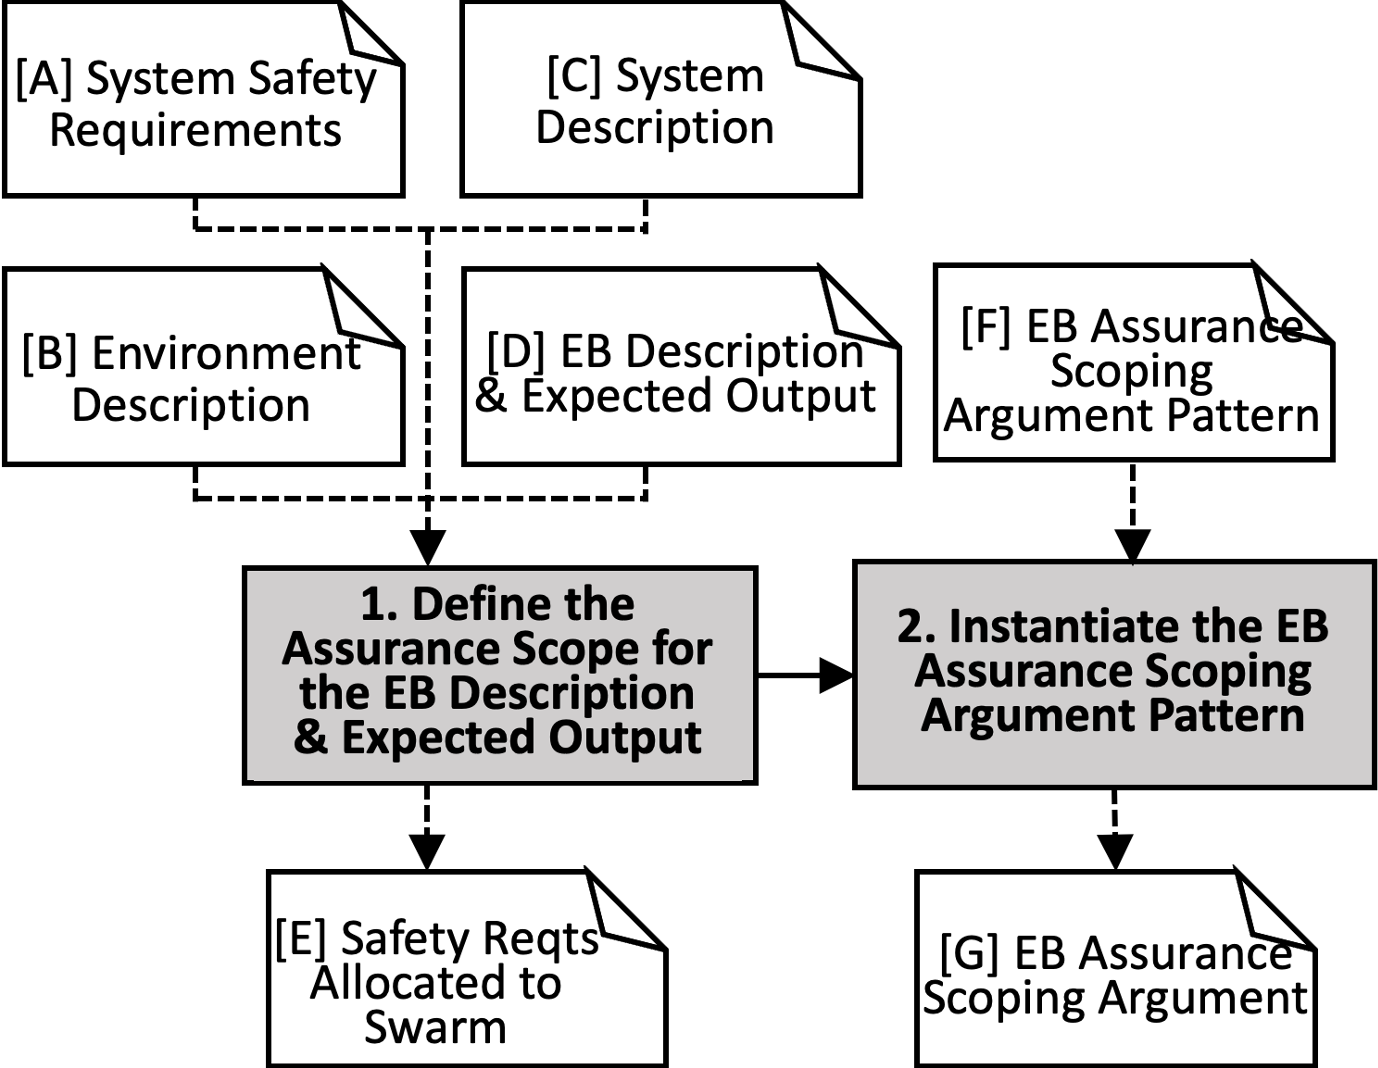
\includegraphics[width=0.99\textwidth]{figures/AERoS-Stage1-v2.png}
%		\vspace{-4ex}%-2ex
%		\caption{Stage 1: The AERoS emergent behaviour assurance scoping process.}
%		\label{amlas-a-stage1}
%	\end{minipage}%
%	\hspace*{.03\textwidth}
%	\begin{minipage}[b]{.5\textwidth}
%		%\centering
%		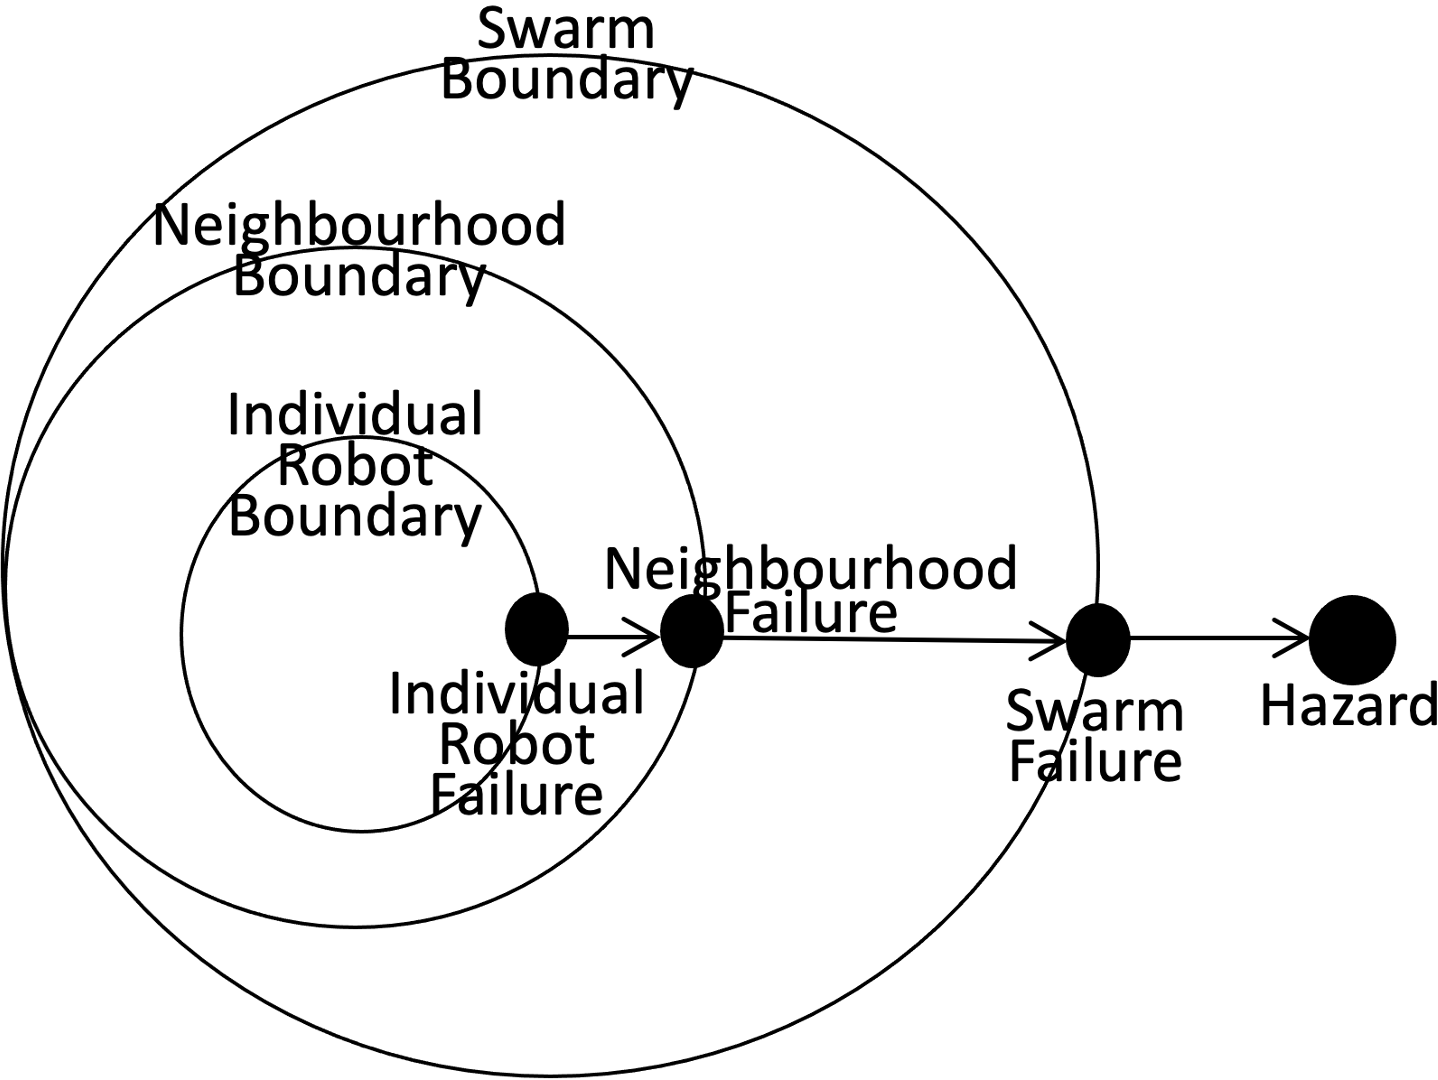
\includegraphics[width=0.99\textwidth]{figures/stage1-failureevents-v4.png}
%		\vspace{-4ex}%-2ex
%		\caption{Failure conditions in a swarm adapted from DO-178C and AMLAS.}
%		\label{failure-events}
%	\end{minipage}
%	\vspace{-6ex} % 4ex
%\end{figure}

\emph{[C] System Description:}
In the cloakroom, we can consider three inputs: sensor availability, neighbourhood data (used because there is no access to global data in real-world deployments), and swarm parameters (see Fig.~\ref{system-description}). 
%In the cloakroom, we can consider three inputs: sensor availability, neighbourhood data, and swarm parameters (see Fig.~\ref{system-description}). 
The \emph{sensors} available to agents can be cameras and laser time-of-flight sensors. 
%The neighbourhood data of the swarm can be specified through the communication systems available to agents (Bluetooth).  
The neighbourhood data of the swarm can be specified through the communication systems available to agents, in this case Bluetooth. 
Through the use of this short-range communication, agents can access neighbourhood data, such as approximate position or current state of local agents.  
As for the swarm-level parameters, we can consider options specified by a user, that is, the number of agents deployed, and the maximum speed of agents. 
Once defined, the three inputs are then fed to the individual agents to instruct their behaviour. This behaviour enacted by multiple agents then produces a swarm-level EB as the individuals interact with one another and their environment. 
%Page 4 - "why single out neighbourhood data?" - emphasize that this is due to communications limitations i.e. we are not assuming access to global data as that would not be available in real-world deployment.

\emph{[D] EB Description and Expected Output:}
By expected output, we refer to the gains that can arise from the system by deploying multiple agents. 
In the cloakroom, the output is a collaborative system capable of collecting, sorting, and delivering jackets in a public setting. 
To achieve this, the EB of the system needs to %be manually engineered <KIE: We say in the abstract that we don't explicitly engineer behaviours of the swarm.
arise from the available behaviours of the individual agents, their interactions, and the constraints outlined in the system description.

\noindent\textbf{Activity 2. Instantiate EB Assurance Scoping Argument Pattern} Each stage of the AERoS process includes an activity to instantiate a safety argument pattern based on the evidence and artefacts generated in that stage. %, following AMLAS~\cite{Hawkins2021}. 
\emph{Argument patterns}~\cite{Hawkins2021}, which are modelled using the Goal Structuring Notation, can be used to explain the extent to which the evidence supports the relevant EB safety claims.  
%GSN is widely used graphical notation to capture safety cases.  
In Activity 2, we use the artefacts generated from Stage 1 (i.e. [A–E]) to instantiate the EB Assurance Scoping Argument Pattern ([F] – see Fig.~\ref{stage1-ap}). 
The instantiated argument [G] along with other instantiated arguments resulting from the other five stages of AERoS constitute the safety case for the swarm. The activities to instantiate argument patterns of the other stages follow a very similar pattern so are not shown due to space limitations.
\begin{figure}[!t]
	\vspace{-1ex}
	\centering
	\begin{minipage}[b]{.45\textwidth}
		\centering
		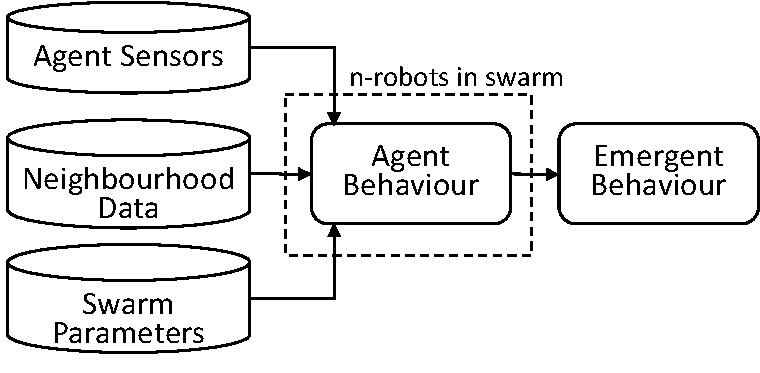
\includegraphics[width=0.99\textwidth]{figures/stage1-systema-v2.pdf} %stage1-systema-v2.png
		\caption{Inputs fed into individual agent behaviour producing overall swarm emergent behaviour. }%{System description.}
		\label{system-description}
	\end{minipage}%
	\hspace*{0.03\textwidth}
	\begin{minipage}[b]{.52\textwidth}
		\centering
		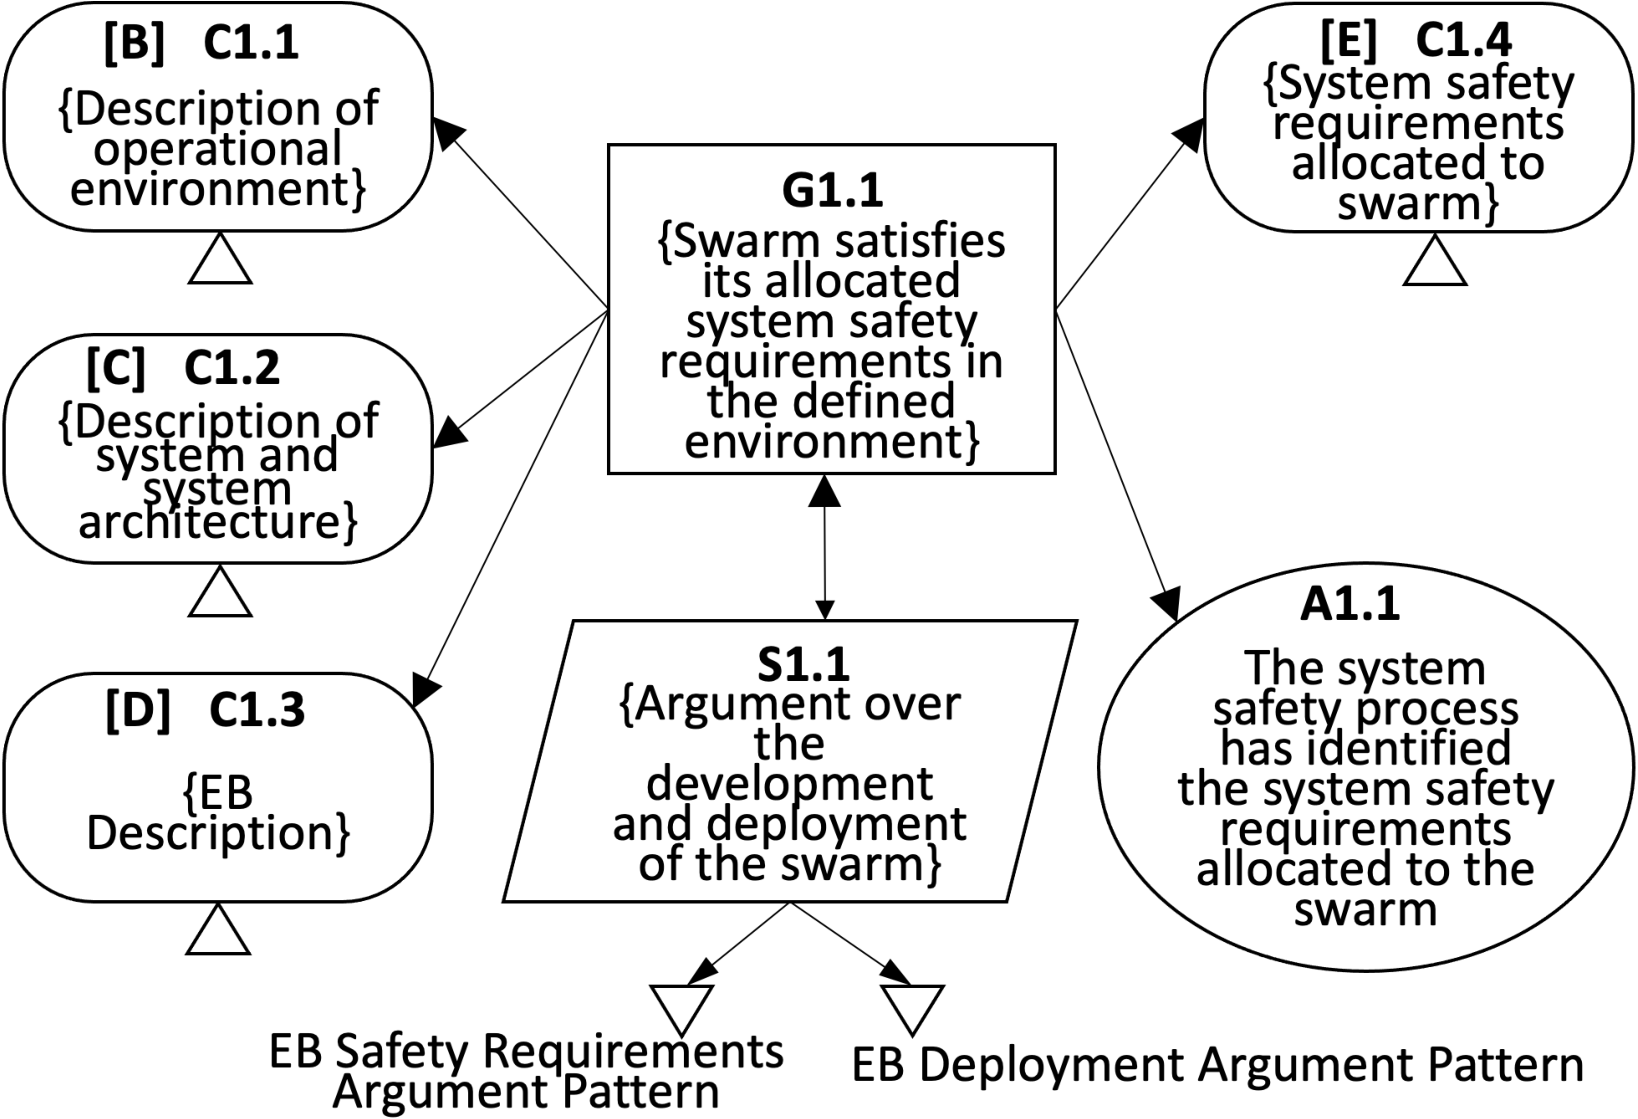
\includegraphics[width=0.99\textwidth]{figures/stage1-argumentpattern-v3.pdf}%stage1-argumentpattern-v2.pdf
		\vspace{-2ex}
		\caption{Emergent behaviour safety assurance scoping argument pattern.}
		\label{stage1-ap}
	\end{minipage}	
	\vspace{-4ex}
\end{figure}
%\begin{figure}[!t]
%	\centering
%	\begin{minipage}[b]{.45\textwidth}
%		\centering
%		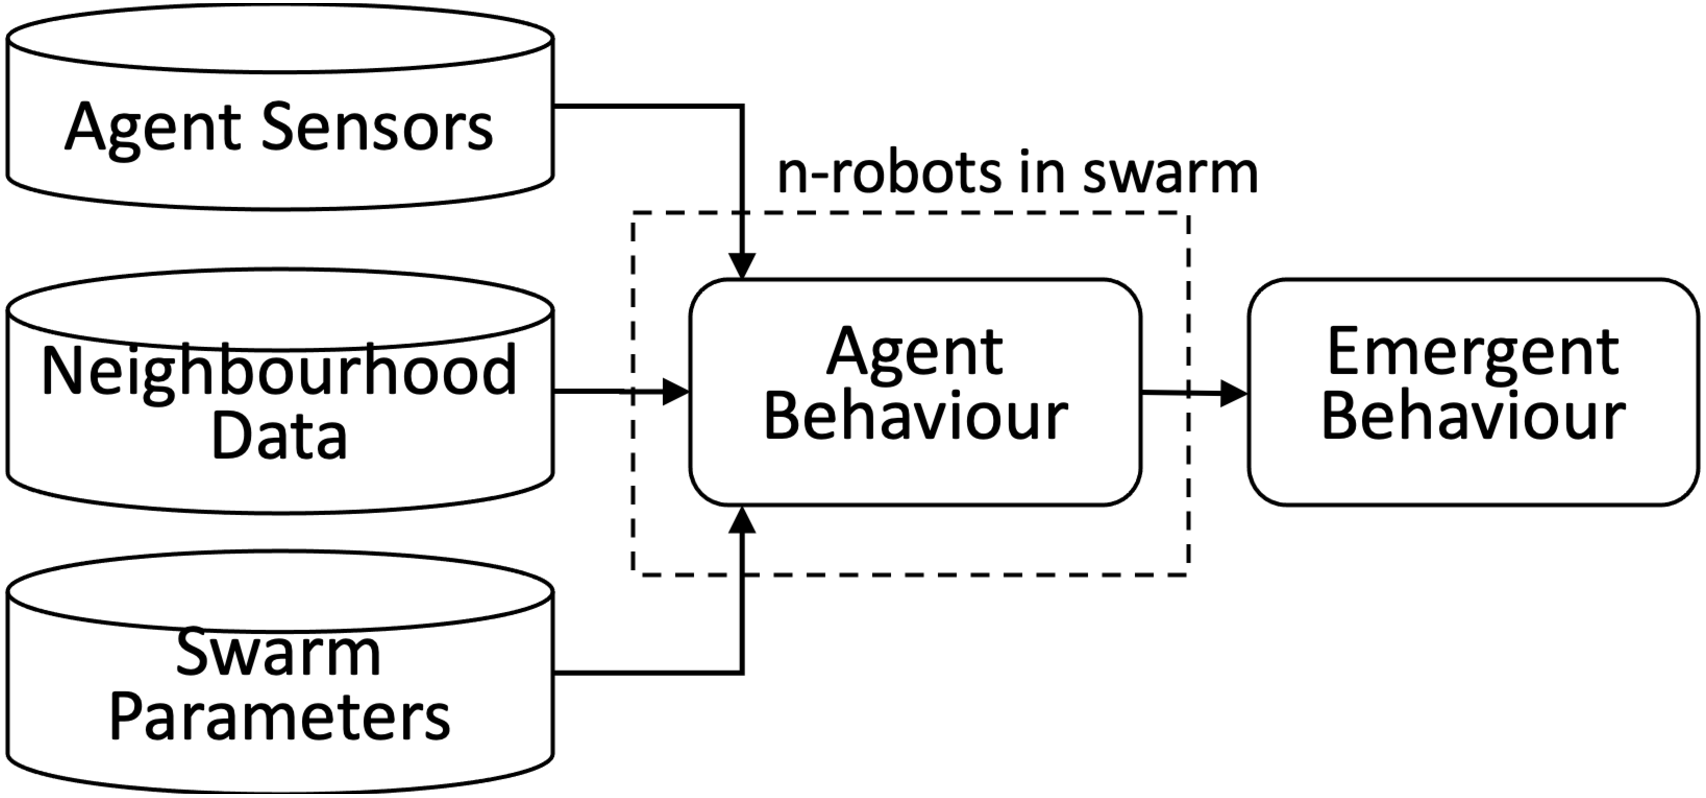
\includegraphics[width=0.99\textwidth]{figures/stage1-systema.pdf} %stage1-systema-v2.png
%		\caption{Inputs fed into individual agent behaviour producing overall swarm emergent behaviour. }%{System description.}
%		\label{system-description}
%	\end{minipage}%
%	\hspace*{0.03\textwidth}
%	\begin{minipage}[b]{.52\textwidth}
%		\centering
%		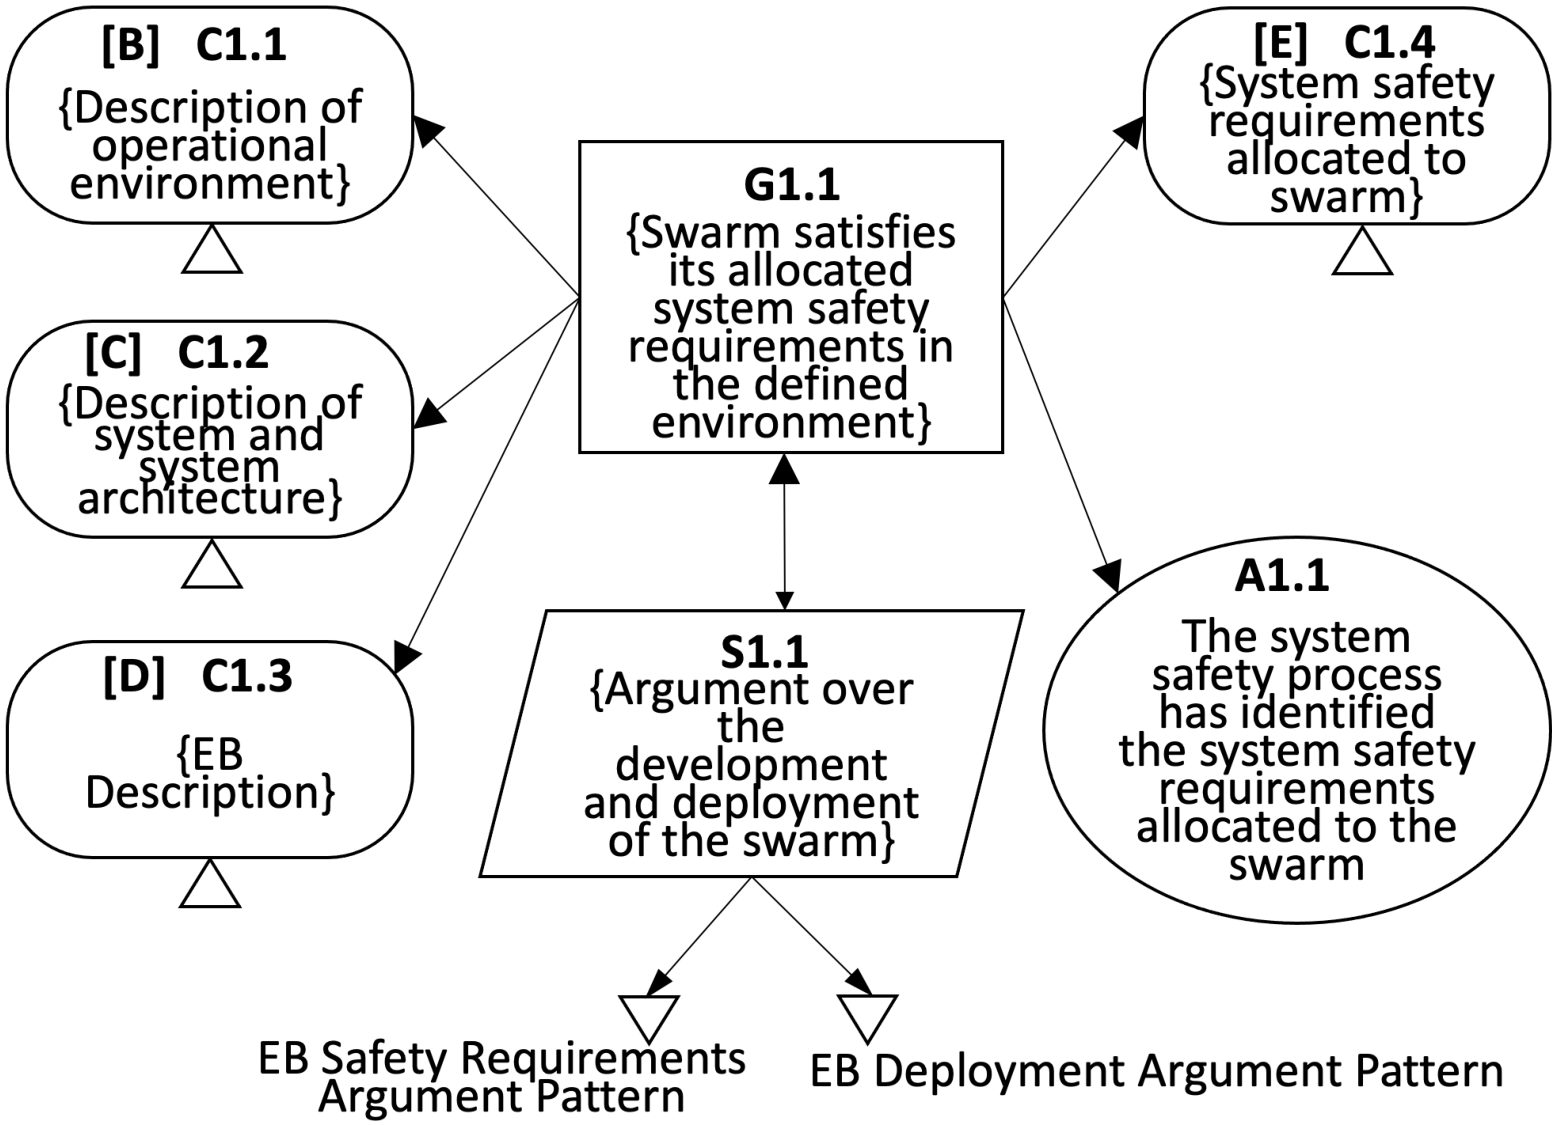
\includegraphics[width=0.99\textwidth]{figures/stage1-argumentpattern-v2.pdf}%stage1-argumentpattern-v3.png
%		\vspace{-2ex}
%		\caption{Emergent behaviour safety assurance scoping argument pattern.}
%		\label{stage1-ap}
%	\end{minipage}	
%	\vspace{-4ex}
%\end{figure}
\subsection{Stage 2: EB Safety Requirements Assurance} \label{framework-stage2}
Stage 2 contains three activities (Fig.~\ref{amlas-a-stage2}), which are performed to provide assurance in EB safety requirements for the swarm. 
%The scope of this stage is limited to the EB model of the swarm.

\noindent\textbf{Activity 3. Develop EB Safety Requirements} %The input to Activity 3 in Stage 2 is the Safety Requirements Allocated to the Swarm [E]. 
We define EB safety requirements to specify risk controls for the swarm-level hazards by taking into account the system architecture defined and the operating environment. 

In the swarm context, we consider four types of requirements: \emph{performance}, \emph{adaptability}, \emph{human safety}, and \emph{environment}. 
Taking inspiration from AMLAS, these requirement types are primarily safety focussed, but we go beyond the performance and robustness safety concerns of ML systems to take into account the swarm operations in a real-world environment. 
The environment requirements capture the need for the system to be robust to variation in the operative space. %swarm related properties.  
%These requirements are all safety related but we go beyond performance and robustness concerns of AMLAS which are typical in ML systems.
We consider several safety metrics under each requirement category: 
(i) performance: low-impact and high-impact collisions (the swarm should operate below a \emph{critical number} of such collisions); %\todo{KIE removed ``...have the ability to avoid...''}
(ii) adaptability: percentage of swarm stationary outside of the delivery site, number of stationary agents, time since last agent moved; 
(iii) human safety: velocity or average velocity of agents, swarm size, rate of humans encountered, proximity to humans;
(iv) environment: sum of objects in an area (the density of objects in the environment should not block swarm operation).
As the robot swarm is composed of many agents, there is potential for a large number of faults to occur at any given time~\cite{Lee2022}. This motivates three further sub-categories for each of the performance, adaptability, and human-safety requirements: \emph{faultless operations}, \emph{failure modes (graceful degradation)}, and \emph{worst case}. 
%\emph{Graceful degradation} refers to the acceptable level of faults, their impact, and how the system should react when faults occur. \emph{Worst case} accounts for the least acceptable impact the system should experience and the means to avoid it. 
%A key output of Activity 3 is [H], which describes the EB Safety Requirements relating to: performance, adaptability, and environment (see Table~\ref{tab:reqs}), as well as human safety (Table~\ref{tab:human-s}). 
A key output of Activity 3 is [H], which describes the EB Safety Requirements relating to: performance, adaptability, environment, and human safety (see Table~\ref{tab:reqs}).  
These example requirements have been generated following three main considerations: the hazards for each safety requirement type, the metrics~\cite{Lee2022} available to assess these hazards, and the realistic thresholds~\cite{Jones2022} given the specification of the system.

% Comments by I.H. on 26/02/2023:
%How were these generated? Rationale?
%Where do these metrics come from and how are they traced to the outcome of the risks analysis? (same questions for the next tables )

%We generate a non-exhaustive set of example requirements following three main considerations: i) the hazards for each safety requirement type; ii) the metrics available in the scenario to assess these hazards, and iii) realistic thresholds given the specification of the system. 

\begin{figure}[t]
	\centering
	\begin{minipage}[b]{.53\textwidth}
		\centering
		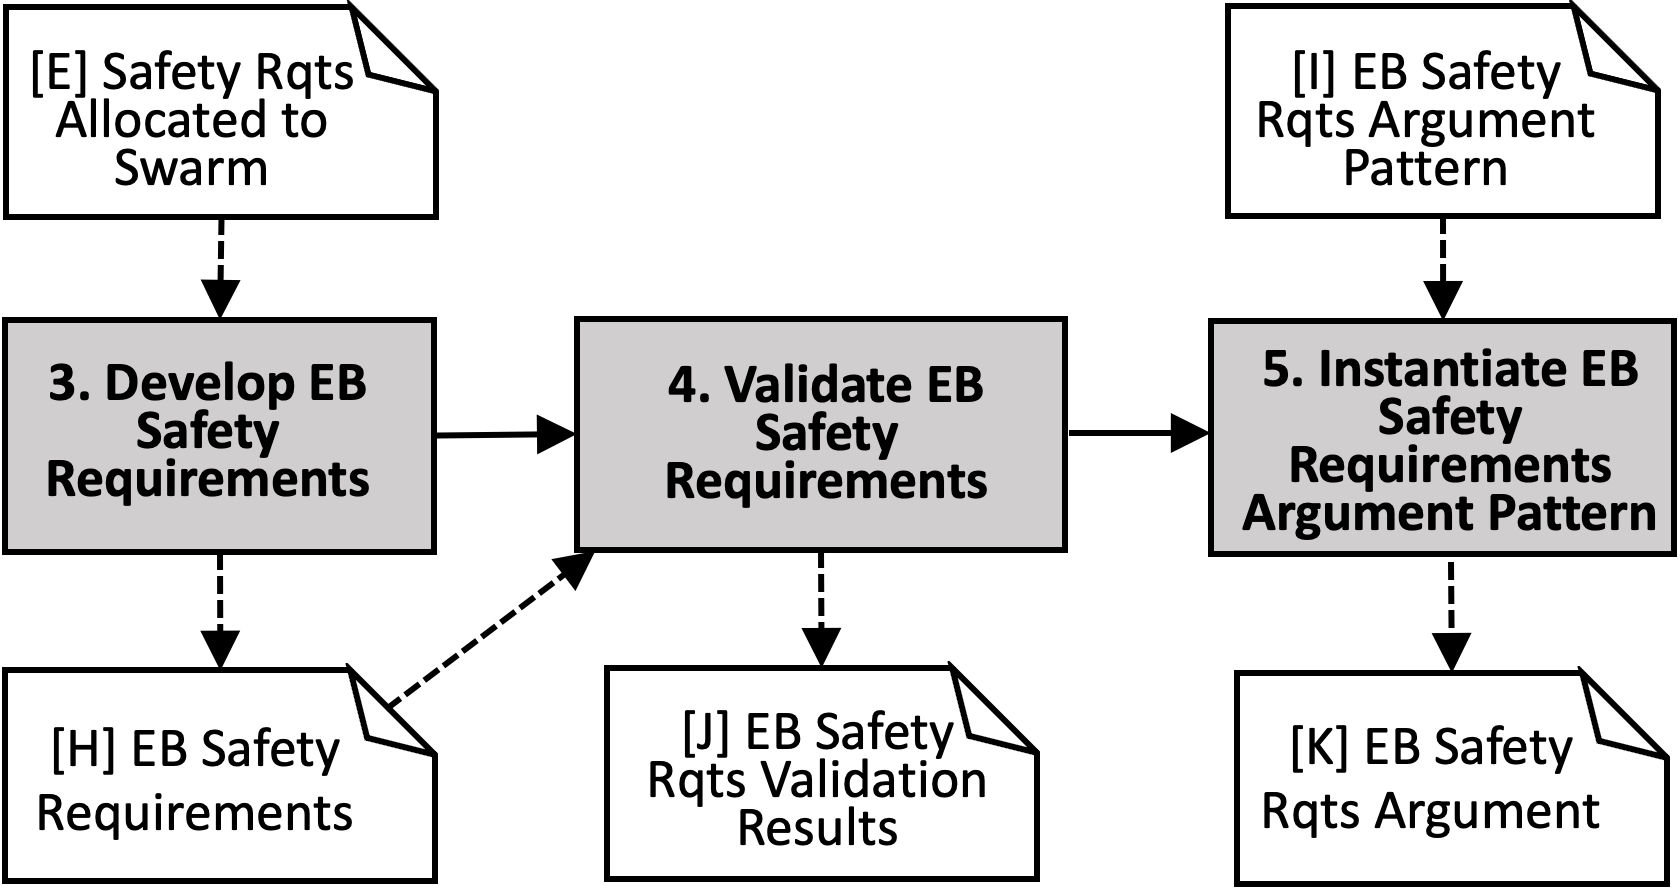
\includegraphics[width=0.99\textwidth]{figures/AERoS-Stage2.png}%amlas-a-stage2-v3.png}
	\vspace{-2ex}
	\caption{Stage 2: The AERoS emergent behaviour safety requirements assurance.}% process.}
\label{amlas-a-stage2}
\end{minipage}%
\hspace*{0.03\textwidth}
\begin{minipage}[b]{.37\textwidth}
\centering
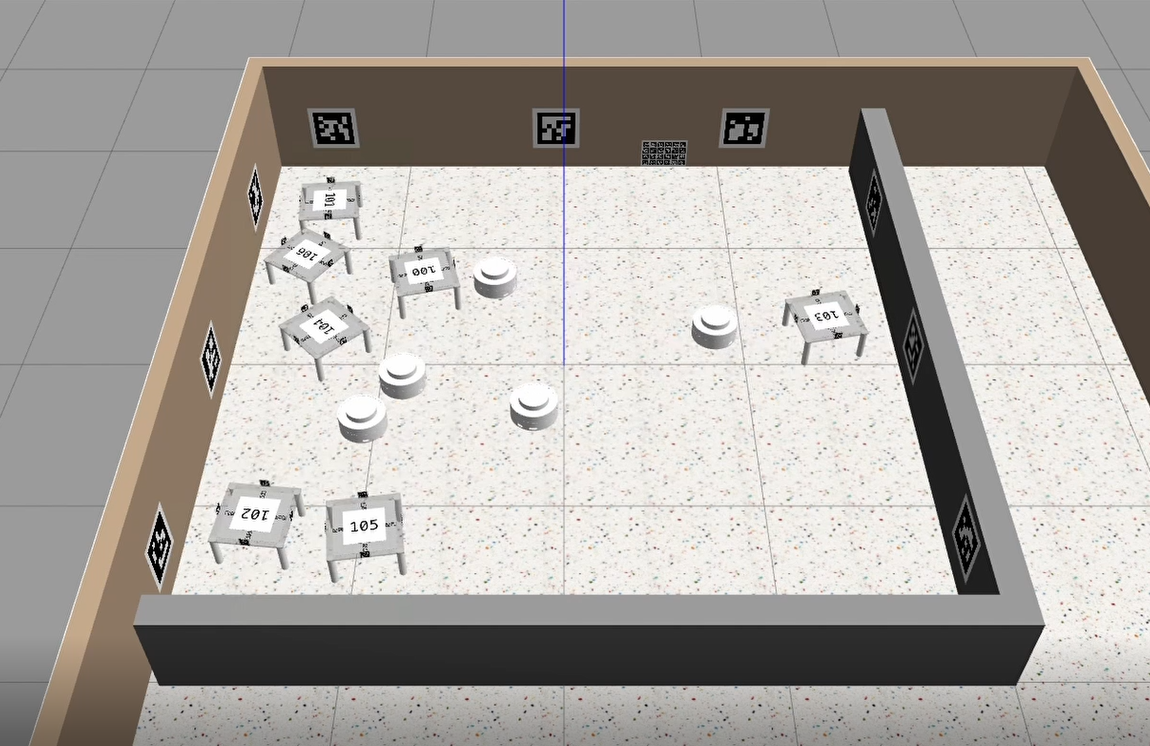
\includegraphics[trim={30mm 25mm 45mm 30mm},clip,width=0.99\textwidth]{figures/3Dsim.png}
\vspace{-2ex}
\caption{3D simulation created to validate several emergent behaviour safety requirements.}
\label{3Dsim}
\end{minipage}
\vspace{-4ex}
\end{figure}
%\begin{figure}[t]
%	\centering
%	\begin{minipage}[b]{.53\textwidth}
%		\centering
%		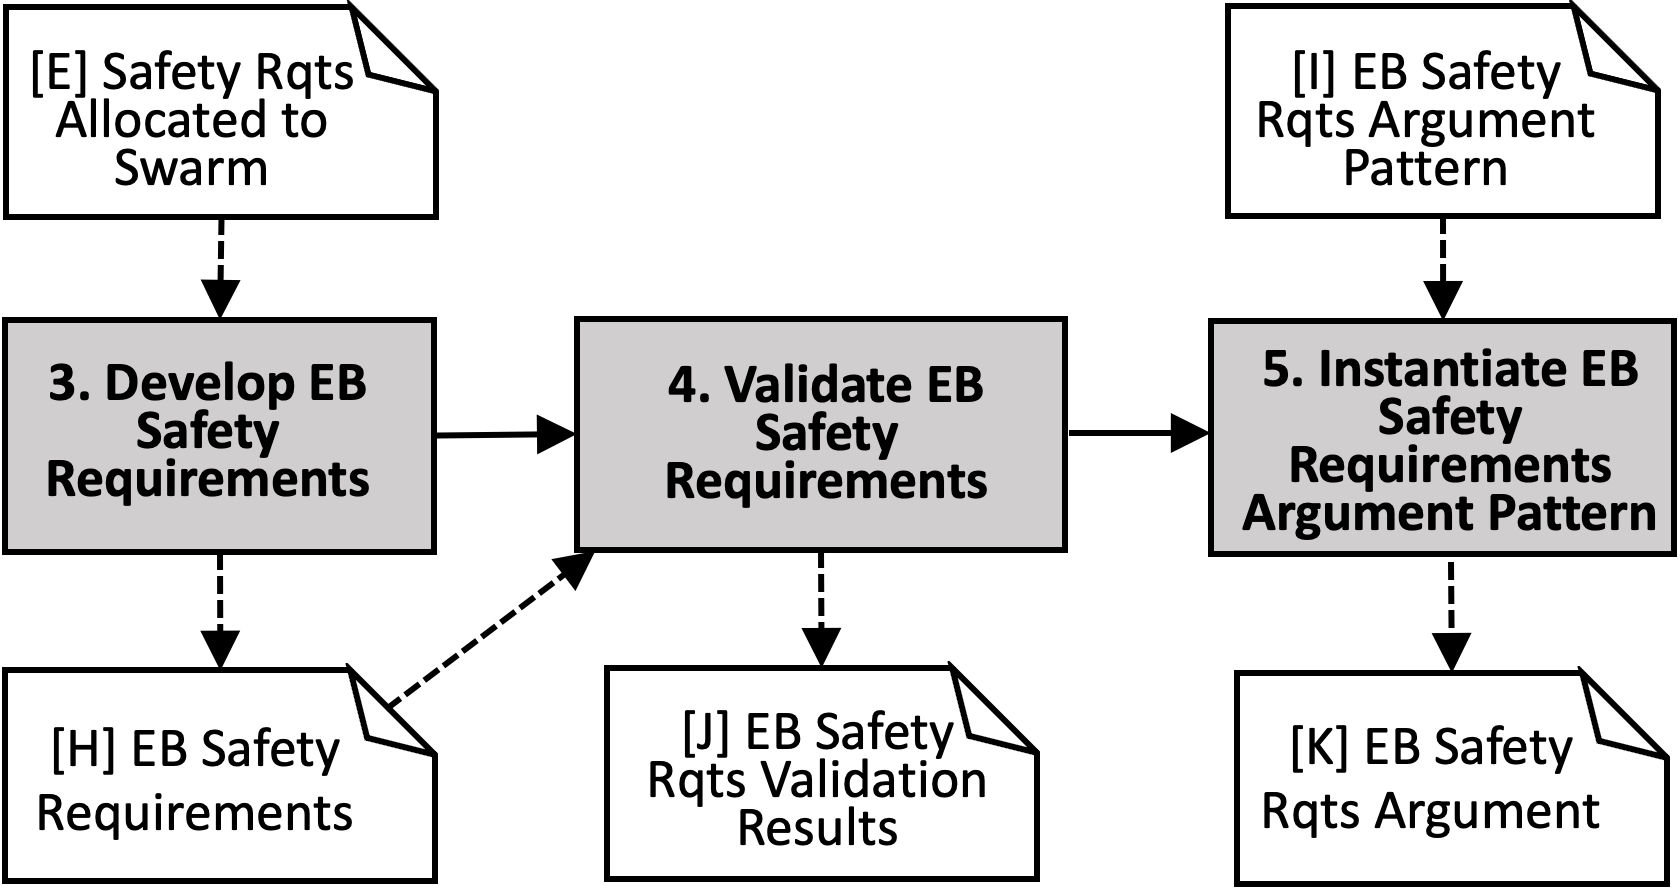
\includegraphics[width=0.99\textwidth]{figures/AERoS-Stage2.png}%amlas-a-stage2-v3.png}
%	\vspace{-2ex}
%	\caption{Stage 2: The AERoS emergent behaviour safety requirements assurance.}% process.}
%\label{amlas-a-stage2}
%\end{minipage}%
%\hspace*{0.03\textwidth}
%\begin{minipage}[b]{.37\textwidth}
%\centering
%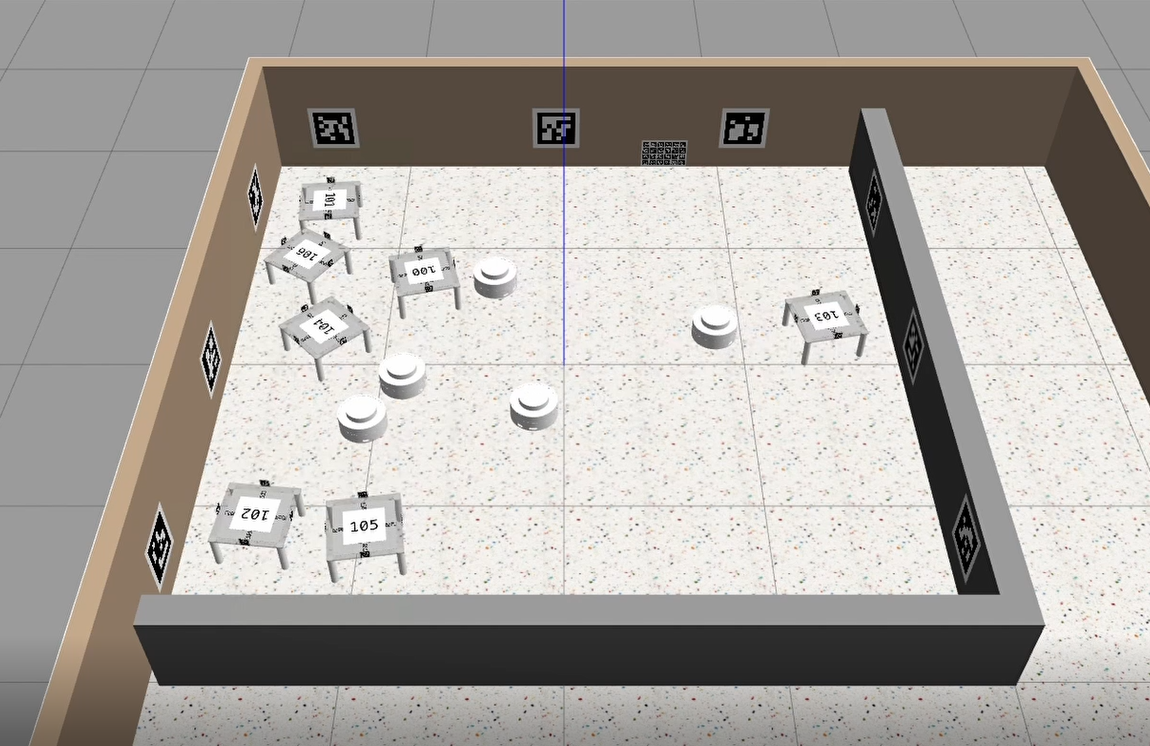
\includegraphics[trim={30mm 25mm 45mm 30mm},clip,width=0.99\textwidth]{figures/3Dsim.png}
%\vspace{-2ex}
%\caption{3D simulation created to validate several emergent behaviour safety requirements.}
%\label{3Dsim}
%\end{minipage}
%\vspace{-2ex}
%\end{figure}
\begin{table}[!t]
	\centering
	\caption{Examples of performance, adaptability, environmental, and human-safety safety requirements for the cloakroom scenario.}
	%\vspace{-2ex}
	\label{tab:reqs}
	\begin{tabular}{p{5mm} p{125mm} }%p{120mm} }
		\textbf{RQ} & \textbf{Performance Requirements}\\
		\hline
		1.1 & The swarm \emph{shall} experience \textbf{$<$ 1 high-impact (V $>$ 0.5m/s)} collisions across \textbf{a day} of \textbf{faultless} operation. \\ 
		\hline
		1.2 & The swarm \emph{shall} experience \textbf{$<$ 0.1\%} increase in \textbf{high-impact} collisions across \textbf{a day's} operation with \textbf{full communication faults} occurring in \textbf{10\%} of the swarm.\\ 
		\hline
		1.3 & The swarm \emph{shall} experience \textbf{$<$ 0.1\%} increase in \textbf{high-impact} collisions across \textbf{a day's} operation with \textbf{half-of-wheels motor faults} occurring in \textbf{50\%} of the swarm.	\\	
		\hline
		1.4 & The swarm \emph{shall} experience \textbf{$<$ 2 high-impact (V $>$ 0.5m/s)} collisions across \textbf{a day} of \textbf{faulty} operation.  \\		 		
		\hline
        1.5 & The swarm agents \emph{shall} \textbf{weigh $<$ 3kg} and shall have \textbf{acceleration} \textbf{$<$ 4m/s} so that the \textbf{maximum collision force} in the swarm is within acceptable bounds. \\
        \hline
        1.6 & The swarm agents \emph{shall} only carry objects of \textbf{weight $<$ 2kg}. \\ 
        \hline \\[-1.25\medskipamount]
		& \textbf{Adaptability Requirements}\\
		\hline
		2.1 & The swarm \emph{shall} have \textbf{$<$ 10\%} of its agents \textbf{stationary*} outside of the \textbf{delivery site} at a given time. *Agents are considered stationary once they have not moved for $>$ \textbf{10s}.
		\\ 
		\hline
		2.2 & All agents of the swarm \emph{shall} move at least every \textbf{100s} if outside of the \textbf{delivery site}.\\ 
		\hline
		2.3 & The swarm \emph{shall} experience $<$ \textbf{10\%} increase in the \textbf{number of stationary agents} at any time with \textbf{half-of-wheels motor faults} occurring in \textbf{50\%} of the swarm. \\
		\hline
		2.4 & The swarm agents \emph{shall} experience $<$ \textbf{10\%} increase in \textbf{stationary time} with \textbf{half-of-wheels motor faults} occurring in \textbf{50\%} of  the swarm.\\ 
		\hline
		2.5 & The swarm \emph{shall} experience $<$ \textbf{10\%} increase in \textbf{number of stationary agents} at any given time with \textbf{full communication faults} occurring in \textbf{10\%} of the swarm.\\
		\hline
		2.6 & The swarm agents \emph{shall} experience $<$ \textbf{10\%} increase in \textbf{stationary time} with \textbf{full communication faults} occurring in \textbf{10\%} of the swarm. \\	
		\hline
		2.7 & The swarm \emph{shall} have \textbf{$<$ 20\%} of its agents \textbf{stationary} outside of the \textbf{delivery site} at a given time. \\ 
        \hline \\[-1.25\medskipamount]
	    & \textbf{Environmental Requirements} \\ 
		\hline
		3.1 & The swarm \emph{shall} perform as required in environmental density levels \textbf{0-4 p$_o$ of objects} (sum of boxes and agents per m$^2$) in the environment. %* p$_o$ = sum of objects / m$^2$.
		\\ 
		\hline
		3.2 & The swarm \emph{shall} perform as required when \textbf{floor incline} is \textbf{0-20 degrees}.
		\\ 
		\hline
		3.3 & The swarm \emph{shall} perform as required in a \textbf{dry environment}.
		\\ 
		\hline \\[-1.25\medskipamount]
		& \textbf{Human-Safety Requirements}\\
	\hline
4.1 & The swarm agents \emph{shall} travel at speeds of less than \textbf{0.5m/s} when within \textbf{2m} distance of a \textbf{trained human} (a worker who has received relevant training).
\\ 
\hline
4.2 & The swarm agents \emph{shall} travel at speeds of less than \textbf{0.25m/s} when within \textbf{3m} distance of an \textbf{attendee}.
\\ 
\hline
4.3 & The swarm agents \emph{shall} only come within \textbf{2m} distance of a \textbf{human $<$ 10} times collectively across \textbf{1000s} of \textbf{faultless} operations.
\\ 
\hline
% 4.4--4.7 removed
%		4.4 & The swarm \emph{shall} only allow \textbf{$<$ 5 agents} to request intervention from a \textbf{trained human} at a given time.
%		\\ 
%		\hline
%		4.5 & A \textbf{trained human} \emph{shall} monitor \textbf{5-20 agents} at a given time.
%		\\ 
%		\hline
%		4.6 & The swarm \emph{shall} only allow \textbf{1 agent} to request input from an \textbf{attendee} at a given time.
%		\\ 
%		\hline
%		4.7 & An \textbf{attendee} \emph{shall} receive  information from $<$ \textbf{5 agents} of the swarm at a given time.
%		\\ 
%		\hline
4.4 & The swarm \emph{shall} experience \textbf{$<$ 10\%} increase in \textbf{human encounters} across \textbf{1000s} of operation with \textbf{full communication faults} occurring in \textbf{10\%} of the swarm. \\
\hline
4.5 & The swarm \emph{shall} experience \textbf{$<$ 10\%} increase in \textbf{human encounters }across \textbf{1000s} of operation with \textbf{half-of-wheels motor faults} occurring in \textbf{50\%} of the swarm.\\
\hline
4.6 & The swarm agents \emph{shall} only come within \textbf{2m} distance of a \textbf{human $<$ 20} times collectively across \textbf{1000s} of \textbf{faulty} operations.
\\				
\hline \\[-1\medskipamount]		
%		\\ 
%		\hline
%		3.4 & The swarm \emph{shall} perform as required in \textbf{smooth-floored environments} with step increases no greater than \textbf{0.5cm}.
%		\\ 
%		\hline
%		3.5 & The swarm \emph{shall} only operate in \textbf{environments where humans have devices that identify the human’s location} to the swarm agents. 
%		\\ 		
%		\hline \\[-1\medskipamount]
	\end{tabular}
\vspace{-4ex}
\end{table}
%\normalsize
%\todo{For 2.2, specify max.\ speed of swarm robots?}
%\todo{Specify the (max.) weight of the entities in the swarm, max.\ power of robots, allows conclusions on impact of forces, e.g.\ when crushing?}
%\todo{Specify max. weight of objects to be moved?}
%\tiny
%
%\normalsize
%A key output of Activity 3 is the EB Safety Requirements [H] which states the safety requirements relating to: performance, adaptability and environment (see Table \ref{tab:reqs}), as well as human safety requirements (see Table \ref{tab:human-s}).
%
%\todo{SW: Not sure of 'injection' phrasing used in table. This is something you would do during testing, but is it the right term for a requirement during operation? Maybe "with 10\% full communication faults within the swarm"}
\noindent\textbf{Activity 4: Validate EB Safety Requirements} The required input to Activity 4 is the EB Safety Requirements [H].  
These
% The EB safety requirements
are validated by both review and simulation.
Firstly, the requirements derived for the cloakroom have been reviewed by a safety-critical systems engineering expert to ensure that the specified EB safety requirements for the swarm will deliver its intended safe operation. Secondly, we validated all safety requirements (excepting RQ3.5 in Table~\ref{tab:reqs}) for the cloakroom system using the Gazebo 3D simulator. 
This simulation is an exact replica of the 4m x 4m lab environment used for hardware implementation (Fig.~\ref{3Dsim}). 
In \textbf{Activity 5}, the artefacts generated in this stage are used to instantiate the EB Safety Requirements Argument Pattern [I].  
\subsection{Stage 3: Data Management} \label{framework-stage3}
When designing EB, input data for training an algorithm comes from local sensing of individual agents, both onboard the agent itself and in its local environment. The activities and outputs in this stage take into account the complexities of interactions between multiple agents.

\noindent\textbf{Activity 6. Define Data Requirements} %In our adaptation of Activity 6, 
We take the EB Safety Requirements [H] outlined in Stage 2 as an input (see Fig.~\ref{amlas-a-stage3}) which guide the data requirements in this activity, feeding into the data specification outlined here. We split the data requirement outputs into two multi-agent focused requirements: [L.0] Data Type Requirements and [L.1] Data Availability Constraints.

%\paragraph*{[L.0] Data Type Requirements}
\emph{[L.0] Data Type Requirements:}
This element focuses on the \emph{relevance}, \emph{completeness}, \emph{accuracy}, and \emph{balance} of the information that will be used to construct the swarm behaviour (see examples in Table~\ref{tab:L0_req}), and subsequently, to test the EB of the system before deployment. The \emph{relevance} of the data used in the development of the EB specifies the extent to which the test environment must match the intended operating domain of the robot swarm. The \emph{completeness} of the data specifies the conditions under which we test the behaviour, that is, the volume of tests that will be run, the variety of tests executed, and the diversity of environments expected to be used in the testing process. The aim is to cover a representative sample of conditions for testing. 
\emph{Accuracy} in this context relates to how well the data captures the parameter space defining the performance of the robot swarm. 
%For example, an accurate dataset for what constitutes a delivery in a logistics scenario~\cite{milner2022stochastic} should track the footprint of a deliverable to ensure it is well-positioned in the delivery zone (RQ7.1). 
\emph{Balance} refers to the evenly distributed trials executed in the testing process of the EB algorithm. % with respect to coverage space. 
By considering balance, we expect the number of tests conducted for failure modes or environments to be justified, ensuring that there is not an unrealistic bias in testing towards a particular scenario. 
%See Table~\ref{tab:L0_req} for examples of data requirements relating to relevance, completeness, accuracy, and balance.
%
%This element focuses on the \emph{relevance}, \emph{completeness}, \emph{accuracy}, and \emph{balance} of the information that will be used to construct the swarm behaviour, and subsequently, to test the EB of the system before deployment. The \emph{relevance} of the data used in the development of the EB specifies the extent to which the test environment must match the intended operating domain of the robot swarm. The \emph{completeness} of the data specifies the conditions under which we test the behaviour, that is, the volume of experiments or tests that will be run, the variety of tests executed, and the diversity of environments expected to be used in the testing process. The aim is to cover a representative sample of conditions for testing. 
%\emph{Accuracy} in this context relates to how well the data captures the parameter space defining the performance of the robot swarm. For example, an accurate dataset for what constitutes a delivery in a logistics scenario~\cite{milner2022stochastic} should track the footprint of a deliverable to ensure it is well-positioned in the delivery zone (RQ7.1). 
%\emph{Balance} refers to the evenly distributed trials executed in the testing process of the EB algorithm. % with respect to coverage space. 
%By considering balance, we expect the number of tests conducted for failure modes or environments to be justified, ensuring that there is not an unrealistic bias in testing towards a particular scenario. See Table~\ref{tab:L0_req} for examples of data requirements relating to relevance, completeness, accuracy, and balance.
%\begin{table}[!t]
%	\centering
%	\caption{\label{tab:human-s}Examples of human-safety requirements for the cloakroom scenario.}
%	\vspace{-2ex}
%	\begin{tabular}{p{6mm} p{130mm}}%p{118mm}}
%	\textbf{RQ} & \textbf{Human-Safety Requirements} \\
%	\hline
%	4.1 & The swarm agents \emph{shall} travel at speeds of less than \textbf{0.5m/s} when within \textbf{2m} distance of a \textbf{trained human} (a worker who has received relevant training).
%	\\ 
%	\hline
%	4.2 & The swarm agents \emph{shall} travel at speeds of less than \textbf{0.25m/s} when within \textbf{3m} distance of an \textbf{attendee}.
%	\\ 
%	\hline
%	4.3 & The swarm agents \emph{shall} only come within \textbf{2m} distance of a \textbf{human $<$ 10} times collectively across \textbf{1000s} of \textbf{faultless} operations.
%	\\ 
%	\hline
%	%		4.4 & The swarm \emph{shall} only allow \textbf{$<$ 5 agents} to request intervention from a \textbf{trained human} at a given time.
%	%		\\ 
%	%		\hline
%	%		4.5 & A \textbf{trained human} \emph{shall} monitor \textbf{5-20 agents} at a given time.
%	%		\\ 
%	%		\hline
%	%		4.6 & The swarm \emph{shall} only allow \textbf{1 agent} to request input from an \textbf{attendee} at a given time.
%	%		\\ 
%	%		\hline
%	%		4.7 & An \textbf{attendee} \emph{shall} receive  information from $<$ \textbf{5 agents} of the swarm at a given time.
%	%		\\ 
%	%		\hline
%	4.8 & The swarm \emph{shall} experience \textbf{$<$ 10\%} increase in \textbf{human encounters} across \textbf{1000s} of operation with \textbf{full communication faults} occurring in \textbf{10\%} of the swarm. \\
%	\hline
%	4.9 & The swarm \emph{shall} experience \textbf{$<$ 10\%} increase in \textbf{human encounters }across \textbf{1000s} of operation with \textbf{half-of-wheels motor faults} occurring in \textbf{50\%} of the swarm.\\
%	\hline
%	4.10 & The swarm agents \emph{shall} only come within \textbf{2m} distance of a \textbf{human $<$ 20} times collectively across \textbf{1000s} of \textbf{faulty} operations.
%	\\				
%	\hline \\[-1\medskipamount]
%\end{tabular}
%\vspace{-6ex}%	\vspace{-4ex}
%\end{table} 

\begin{figure*}[!t]%[!ht]
	\centering
	\vspace{-1ex} % -
	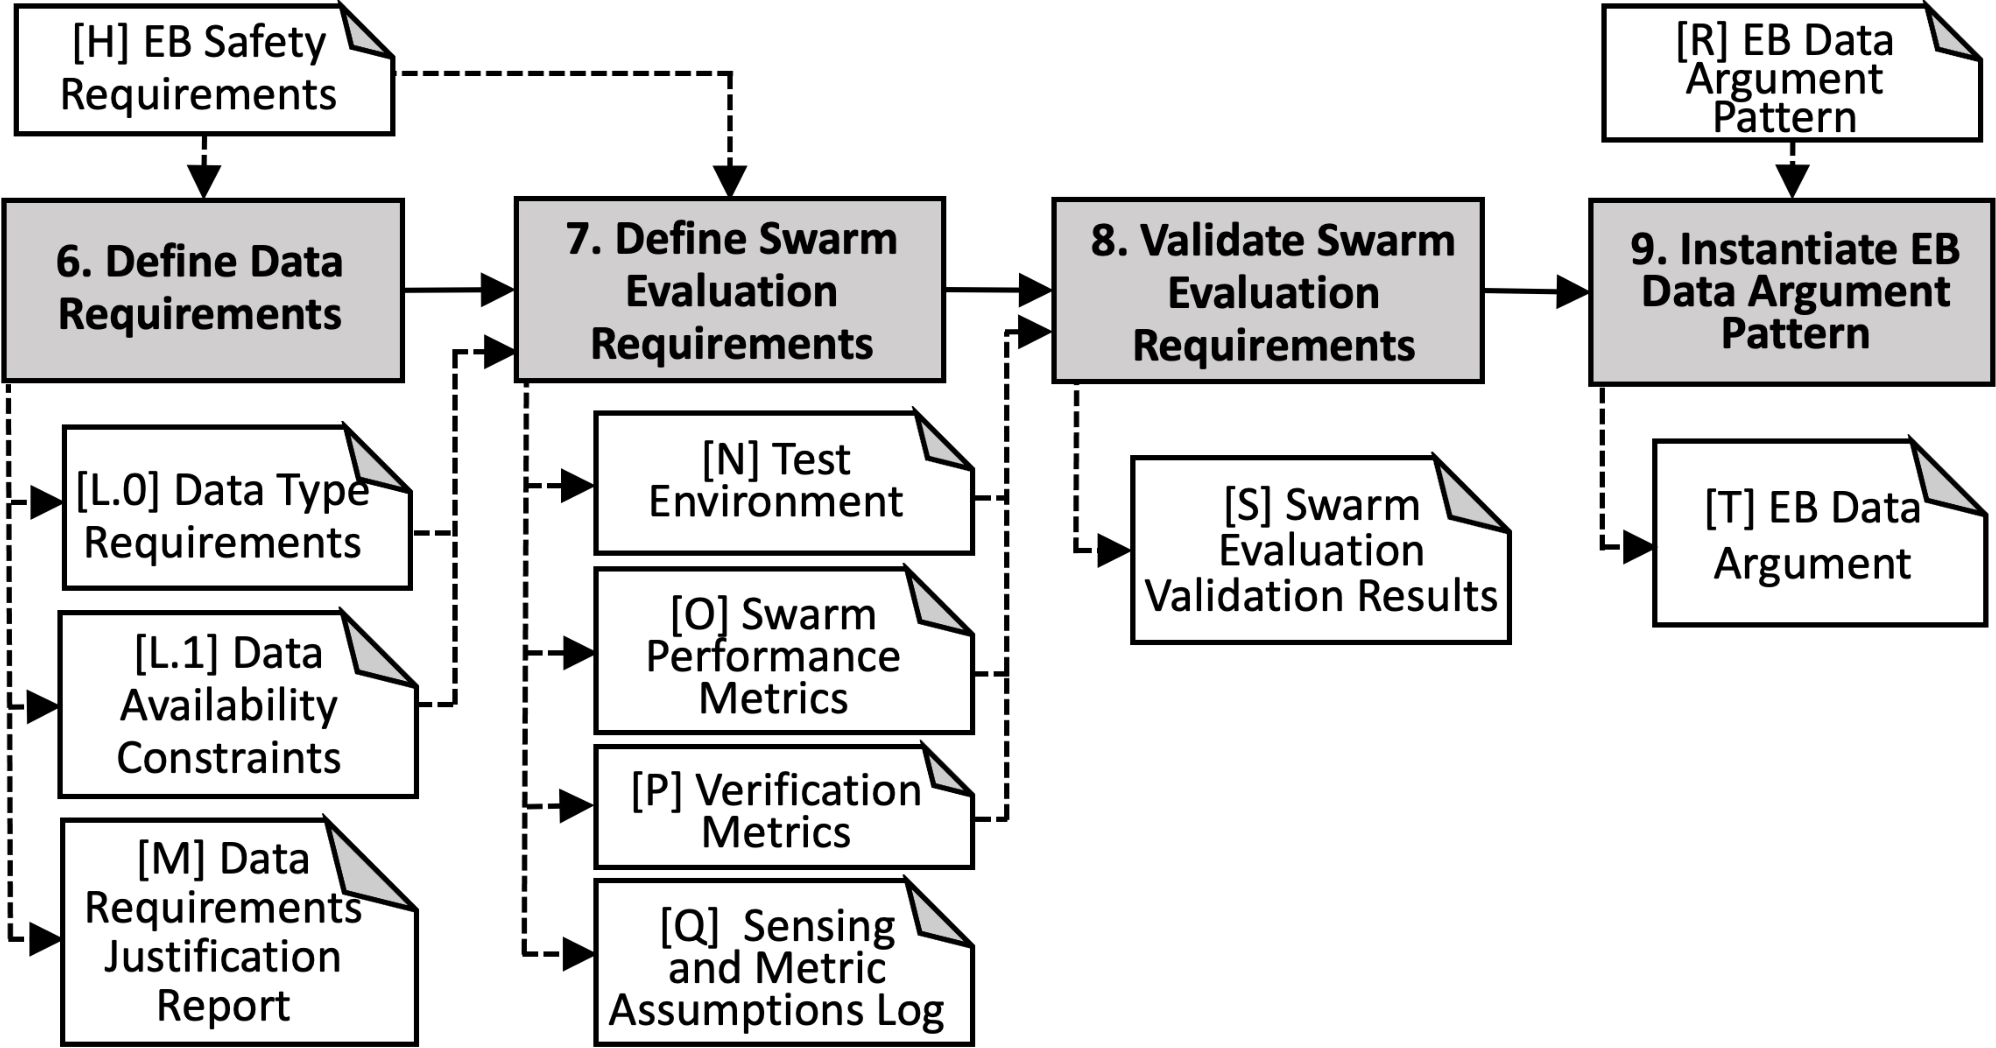
\includegraphics[width=0.75\textwidth]{figures/AERoS-Stage3-V2.pdf}%width=0.75    AERoS-Stage3
	\vspace{-2ex} % 2
	\caption{Stage 3: The AERoS data management process.}
	\label{amlas-a-stage3}
	\vspace{-4ex} % 4
\end{figure*}
%\begin{figure*}[!b]%[!ht]
%	\centering
%	\vspace{-5ex} % -
%	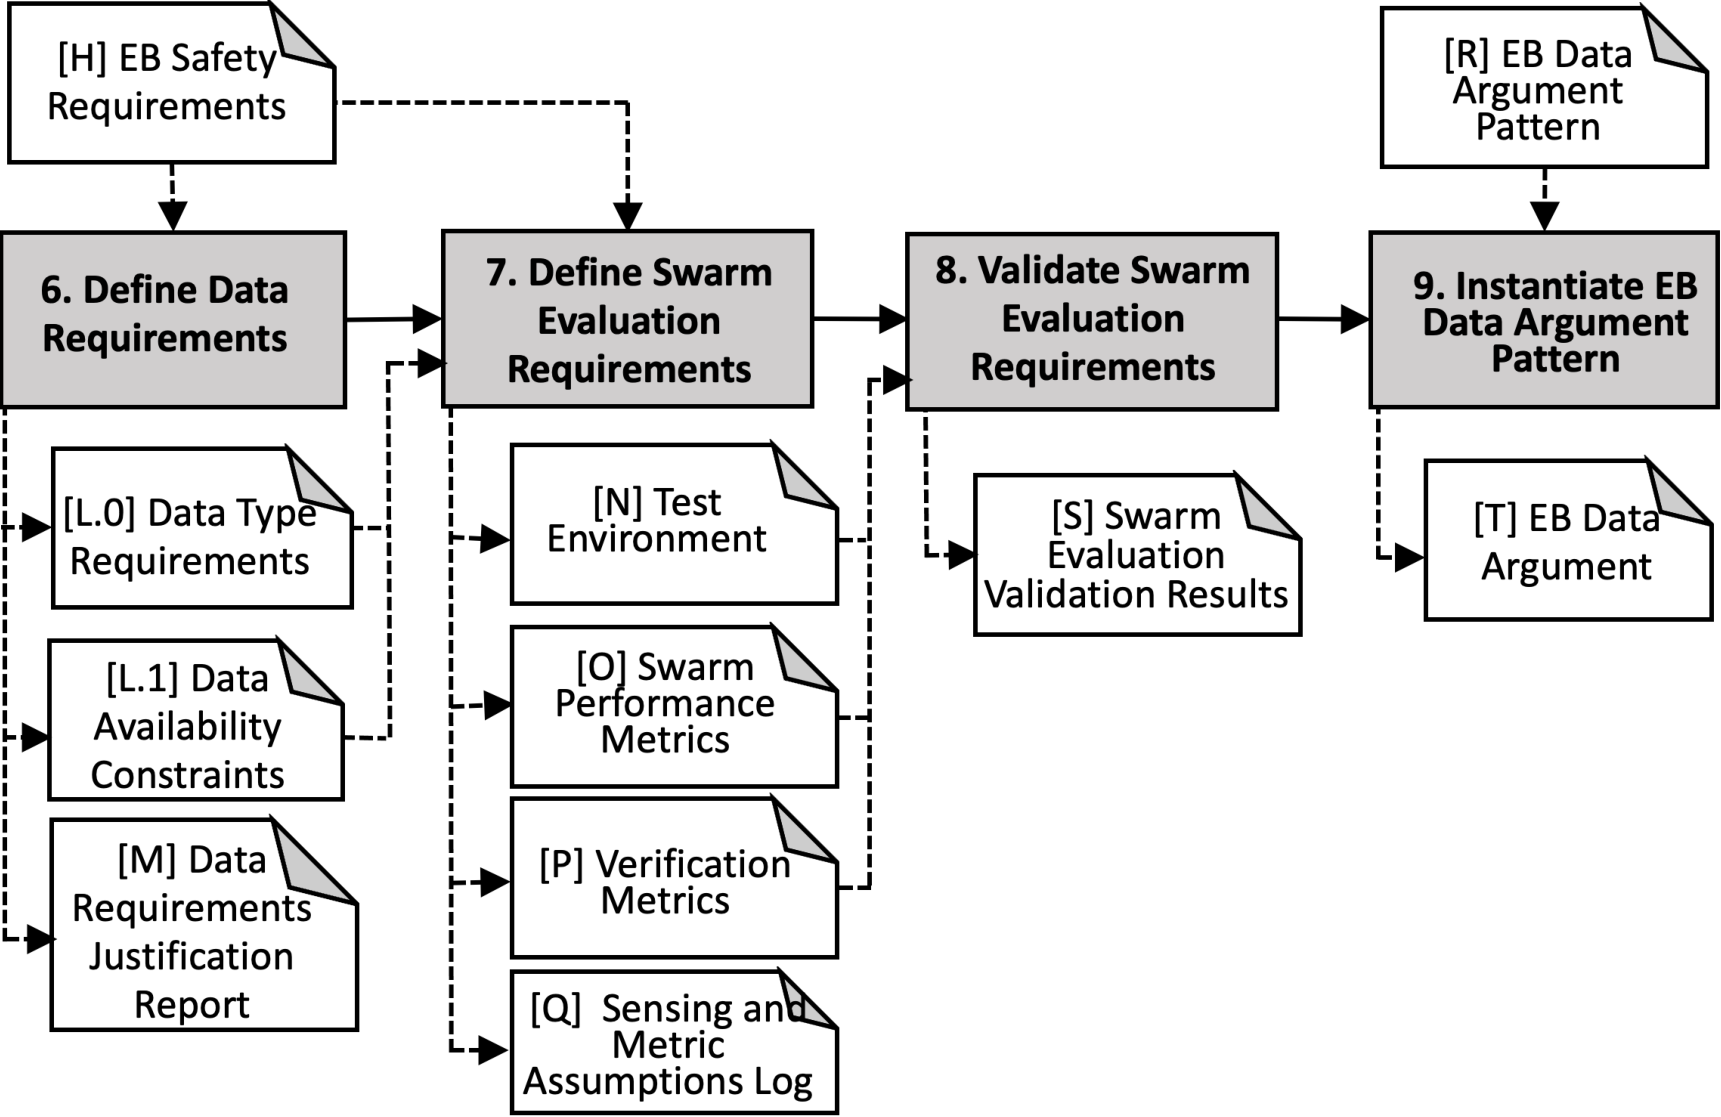
\includegraphics[width=0.75\textwidth]{figures/AERoS-Stage3.pdf}%width=0.75 
%	\vspace{-2ex} % 2
%	\caption{Stage 3: The AERoS data management process.}
%	\label{amlas-a-stage3}
%	\vspace{-4ex} % 4
%\end{figure*}

\emph{[L.1] Data Availability Constraints:}
With the introduction of multiple agents comes the issue of data availability. Distributed communication is a key feature found in emergent systems. As such, it is crucial to define how much information each agent is expected to hold, how easily data may transfer between agents, and across what range agents should be able to transfer information between one another. 
Feasible constraints include \emph{storage capacity}, \emph{available sensors}, \emph{communication range} and \emph{operator feedback}~\cite{Jones2022}.  
%Feasible constraints include~\cite{Jones2022}: (i) \emph{storage capacity: }the swarm agents \emph{shall} have a maximum of 2 GB of information stored on board at any time; (ii) \emph{available sensors:} the swarm agents \emph{shall} only have access to environmental data deemed feasibly collectable by radially positioned cameras and laser time-of-flight sensors; (iii) \emph{communication range:} the swarm agents \emph{shall} only have access to other agent data when within communications range of 5 metres; and (iv) \emph{operator feedback:} the swarm agents \emph{shall} only share information with non-agents (e.g.\ operator terminal) when within communications range of 5 metres.
\begin{table}[!t]%[h]
	\centering
	\caption{Examples of requirements for output [L.0].}
	\vspace{-2ex}
	\label{tab:L0_req}
	\begin{tabular}{p{0.5cm} p{13.4cm}}%p{11.6cm}}
	\textbf{RQ} & \textbf{Relevance Requirements Examples} \\
	\hline
	5.1 & All simulations \emph{shall} include environments with ranges of incline between 0-20\textdegree.\\
	\hline
	5.2 & All simulations \emph{shall} be conducted in a dry environment.\\
	% \hline
	% 5.3 & All simulations shall include floors with step increases that are $\leq$ 0.5 cm.\\
	\hline \\[-1.25\medskipamount]
	& \textbf{Completeness Requirements Examples} \\
	\hline
	6.1 & All simulations \emph{shall} be repeated to include occurrences of faults representative of full communication faults.\\
	\hline
	6.2 & All simulations \emph{shall} be repeated a sufficient number of times to ensure results are representative of typical use.\\
			\hline
			6.3 & All simulations \emph{shall} be repeated in multiple environments representative of those expected in real-world use of the system.\\
	% \hline
	% 6.4 & All simulations shall include sufficient range of robot density levels within the scope of the operational domain.\\ 
	\hline \\[-1.25\medskipamount]
	& \textbf{Accuracy Requirements Examples} \\
	\hline
	7.1 & All boxes \emph{shall} only be considered `delivered’, if all four of the boxes’ feet are positioned within the delivery zone.\\
	\hline
	7.2 & All boxes \emph{shall} only be considered `delivered’, once they are no longer in direct contact with a swarm agent.\\
	\hline \\[-1.25\medskipamount]
	& \textbf{Balance Requirements Examples} \\
	\hline
	8.1 & All simulations \emph{shall} be repeated to obtain representative evaluations for each possible mode of failure (defined under performance, adaptability and human-safety requirements in Stage 2).\\
	\hline
	8.2 & All simulations \emph{shall} be repeated equally across all test environments.\\
	\hline \\[-1\medskipamount] %\hline
\end{tabular}
\vspace{-4ex}%-3ex 
\end{table}

\emph{[M] Data Requirements Justification Report:}
This report is an assessment of the data requirements, providing analysis and explanation for how the requirements and constraints ([L.0] and [L.1]) address the EB Safety Requirements [H].
% This report acts as an assessment of the data requirements, providing analysis and explanation for how the requirements and constraints (outlined in [L.0] and [L.1]) address the EB Safety Requirements specified in [H].

\noindent\textbf{Activity 7. Define Swarm Evaluation Requirements} Taking the outputs [L.0] and [L.1] from Activity 6, the evaluation requirements consider how the EB of the swarm will be assessed, specifying the testing environment and the metrics to be used to assess the test results. %\todo{KIE removed ``comprising''}

\emph{[N] Test Environment:} This takes into consideration the requirements specified in Activity 6, and defines the environment in which the EB will be tested. In most cases this will be multiple simulation environments featuring diverse sets of the terrain, environmental conditions, and obstacle configurations. There may also be instances in which this test environment is specified as a physical environment operating under laboratory conditions, with a hardware system acting as a test bed to observe designed behaviours.

\emph{[O] Swarm Performance Metrics:} This output is used to quantify how well the system is performing. While there may be multiple performance metrics, these metrics should be defined with respect to the primary function of the robot swarm. Metrics that might feature in this output could include: the delivery rate in a logistics scenario, the rate of area coverage in an exploration task, or the response time in disaster scenarios.

\emph{[P] Verification Metrics:} These metrics should be derived from the EB Safety Requirements [H] specified in Stage 2. 
They are intended to be used as the criteria for success within the verification process. 
%Examples of these metrics and their related safety requirements are: swarm density, which is used in verifying environmental safety specifications such as RQ3.1, maximum collision force experienced by agents, which could be used to verify that the swarm meets performance requirements such as RQ1.1 and RQ1.2, or the current speed of all agents, a metric relating directly to the human-safety requirements RQ4.1 and RQ4.2. 
For example, swarm density, which is used in verifying environmental safety specifications such as RQ3.1, maximum collision force experienced by agents, which could be used to verify that the swarm meets performance requirements such as RQ1.1 and RQ1.2, or the current speed of all agents, a metric relating directly to the human-safety requirements RQ4.1 and RQ4.2. 
Identifying [P] early, ideally during the requirements assurance stage, allows consideration of [P] during the design and development of the swarm to facilitate verification.  
%In fact, [P] can be identified and given consideration much earlier, such as during the requirements assurance stage. So, one can design the swarm accordingly and meet the verification criteria at the end.
%In fact, consideration to [P] can be even provided during much earlier stages like the requirements assurance stage. So, one can design the swarm accordingly and meet the verification criteria at the end.
%In fact, one can even provide consideration to [P] during much earlier stages like the requirements assurance stage. So, one can design the swarm accordingly and meet the verification criteria at the end.
%In fact, providing consideration for [P] even much earlier like during the requirements assurance stage is important. So, one can design the swarm accordingly and meet the verification criteria at the end.
%It is important to identify [P] even much earlier stage like Stage 2, so one can design accordingly and meet the verification criteria at the end.
%
%That type it's important to identify these metrics early.
%So that we can design the swarm with these metrics in mind.
%Because that will make it easier to meet the verification criteria in the end.
%
% I.H. Comment: Good point. Also stress here the importance of considering this issue at the requitements stage.
%
%  safety performance requirements -> performance  requirements

\emph{[Q] Sensing and Metric Assumptions Log:} This log serves as a record of the details and decisions made in Activities 6 and 7. It should contain details of the choices made when producing the Test Environment [N], Swarm Performance Metrics [M], and the Verification Metric [P].

\noindent\textbf{Activity 8. Validate Evaluation Requirements} Taking into account outputs [N], [O], and [P] from Activity 7, this activity aims to validate these components with respect to the requirements specified in Activity 6. Should any discrepancies exist between the data requirements and the evaluation requirements, they should be fully justified and recorded in the output Swarm Evaluation Validation Results [S]. 
The artefacts generated in this stage are used to instantiate the EB Data Argument Pattern [R] in \textbf{Activity 9}.

\subsection{Stage 4: Model Emergent Behaviour} \label{framework-stage4}
In the design of an EB algorithm, the challenge is in selecting behaviours at the individual level of the agents which give rise to the desired EB at the swarm level. 
% In the original AMLAS process, Stage 4 focuses on the creation, testing, and instantiation of a machine learning model for a single system with no consideration given to EB for a collective. 
%In our adaptation of AMLAS for the robot swarm,  
We step away from the machine learning paradigm to allow consideration for all possible optimisation algorithms which may attain the target EB.

\noindent\textbf{Activity 10. Create EB Algorithm} 
This can be nature inspired, hand designed, or evolved from a relatively simple set of instructions for individual behaviour, which takes into account agent-to-agent and environmental interactions~\cite{Jones2018}. These instructions when given to a large number of agents, create a synergistic behaviour for the swarm that is more powerful than the sum of the individual agent's performance. 
%The EB algorithm is engineered at the level of the individual agent behaviours for the Test Environment output [N] from Stage 3. The resultant EB must meet the Safety Requirements [H] defined in Stage 2 (see Fig.~\ref{amlas-a-stage4}).
The EB algorithm is engineered at the level of the individual agent behaviours for the Test Environment output [N] from Stage 3. The resultant EB must meet the Safety Requirements [H] defined in Stage 2 (see Fig.~\ref{amlas-a-stage4}) and this will be tested in the following activity. 
In the cloakroom case study, the target EB for the swarm must ensure that items are stored and retrieved by individuals as quickly as possible. An example control algorithm for the individual which produces the desired collective navigation and transport behaviours is a simple random walk \cite{milner2022stochastic}. The swarm engineer may adjust parameters such as robot velocity to optimize for rate of task completion. However, the EB Safety Requirements [H] should eliminate parameter choices which give rise to safety hazards. 
%necessarily constrain the choice of parameters.%possibilities. 
%In the cloakroom case study, the target EB for the swarm must ensure that items are stored and retrieved by individuals as quickly as possible. An example control algorithm for the individual which produces the desired collective navigation and transport behaviours, is a simple random walk \cite{milner2022stochastic}. The swarm engineer may adjust parameters such as robot velocity to optimize for rate of task completion, however, the Safety Requirements [H] necessarily constrain the possibilities. 
%In the cloakroom case study, the target EB for the swarm must ensure that items are stored and retrieved by individuals whilst meeting all requirements specified. 
For example, performance requirements RQ1.1 and RQ1.2 specify an upper bound on the low/high-impact collisions that a swarm shall experience in a given time frame. 
These requirements may be fulfilled by constraining the maximum velocity of individual robots or by ensuring that a robot has one or more sensory devices, such as a camera, enabling it to detect obstacles. 
The key output from this activity is the Candidate EB [U] for testing.
%\todo{SW: Does the Candidate EB Algorithm box need a letter label? Odd to have every other box labelled and not this one.}

%\emph{[V] Model Development Log:} This should log the rationale in the design process of the EB algorithm, in particular how all specified Safety [H] and Data Type Requirements [L.0] have been met given the Data Availability Constraints [L.1].
\emph{[V] Model Development Log:} This should log the rationale in the design process of the EB algorithm, in particular how all Safety [H] and Data Type Requirements [L.0] have been met given the Data Availability Constraints [L.1].

\begin{figure}[!t]
	\centering
	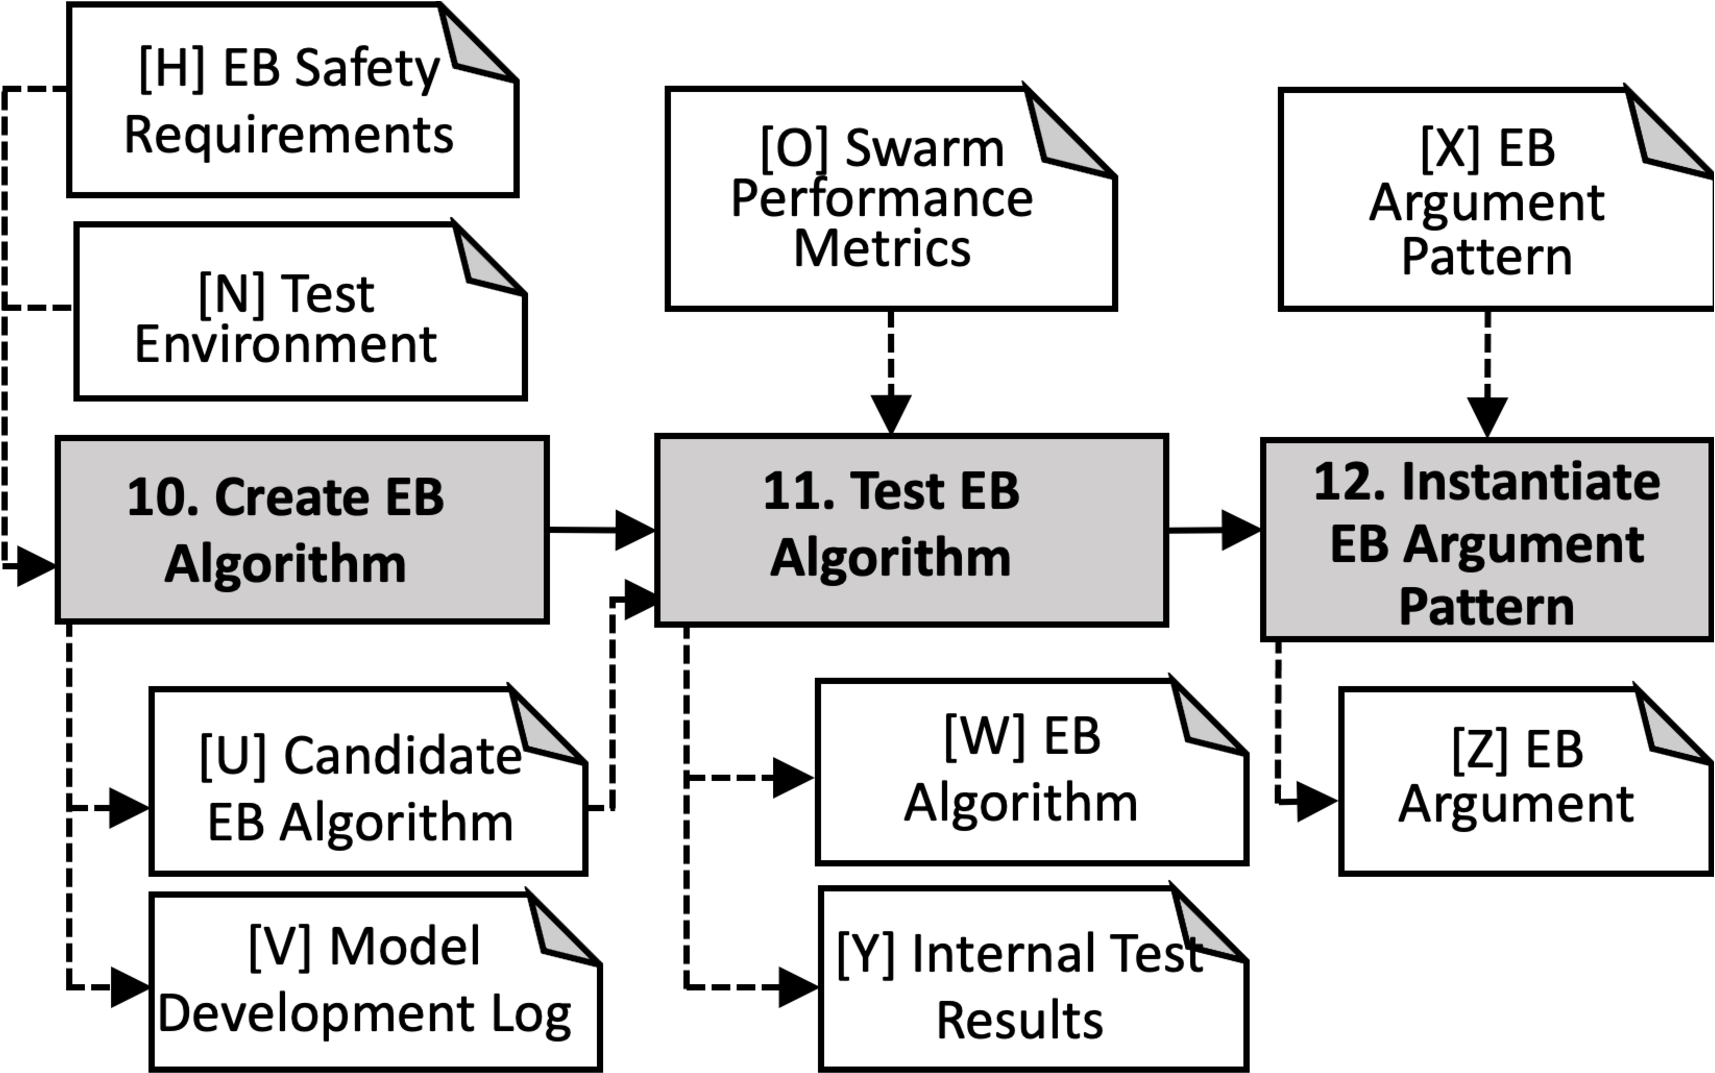
\includegraphics[width=0.55\textwidth]{figures/AERoS-Stage4-V2.pdf}%AERoS-Stage4.pdf %[width=0.55\textwidth]{figures/AERoS-Stage4.pdf}
	\vspace{-2ex}
	\caption{Stage 4: The AERoS model learning process.}
	\label{amlas-a-stage4}
	\vspace{-4ex}
\end{figure}
%\begin{figure}[!t]
%	\centering
%	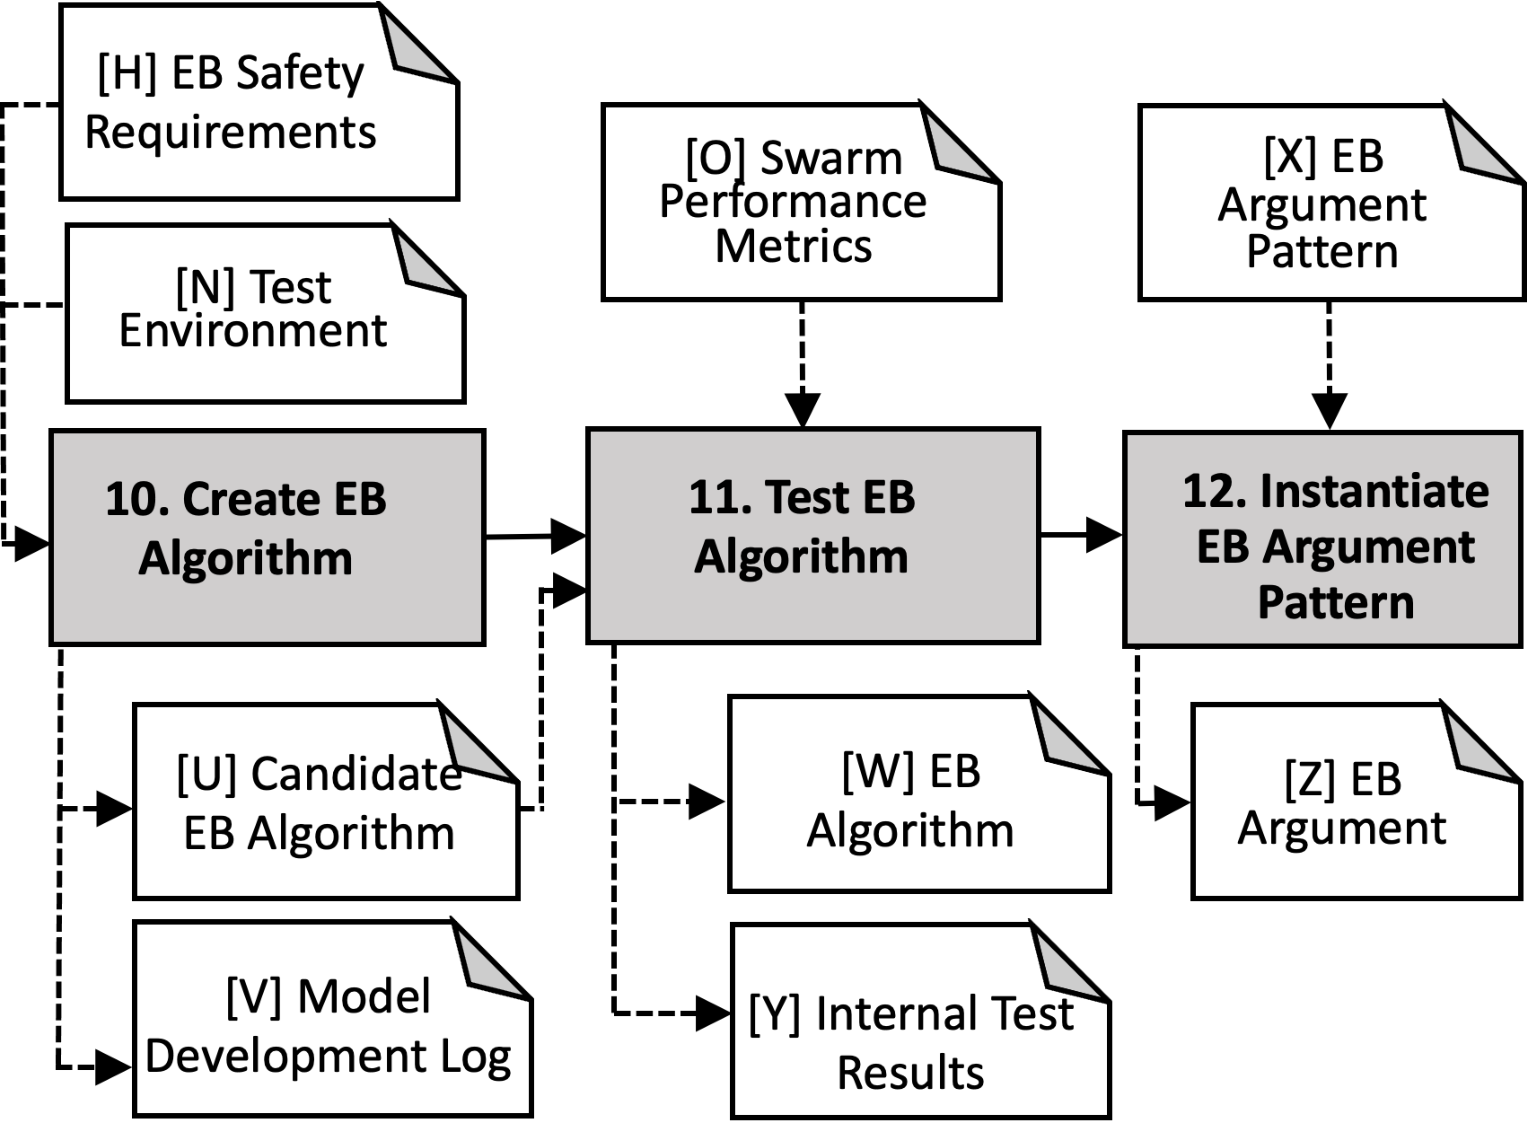
\includegraphics[width=0.55\textwidth]{figures/AERoS-Stage4.pdf}%AERoS-Stage4.png
%	\vspace{-2ex}
%	\caption{Stage 4: The AERoS model learning process.}
%	\label{amlas-a-stage4}
%	\vspace{-4ex}
%\end{figure}

\noindent\textbf{Activity 11. Test EB Algorithm} In this activity, the candidate EB algorithm will be tested against the Swarm Performance Metrics [O] produced in Stage 3. Testing ensures that the Candidate EB Algorithm [U] performs as desired with respect to the defined metrics and in the case where performance passes accepted thresholds, the EB Algorithm [W] will be produced as the output of the activity. If testing fails, [U] can be iteratively modified and tested until it passes successfully.

\emph{[Y] Internal Test Results:} This output provides a degree of transparency in the testing procedure as the results may be further examined to ensure tests have run correctly. 
In \textbf{Activity 12}, the artefacts generated in this stage are used to instantiate the EB Argument Pattern [X].

\subsection{Stage 5: Model Verification} \label{framework-stage5}
\vspace{-0.6ex}
\noindent\textbf{Activity 13. Verify EB} The inputs to the verification process are the EB Safety Requirements [H], Verification Scenarios (Test Generation) [P], and the EB Algorithm [W] (see Fig.~\ref{amlas-a-stage5}). 
%
The verification method and assessment process within that method will be largely determined by the specifics of the safety requirements. Some safety specifications lend themselves towards certain assessment methods due to the scenarios they prescribe.
%
For example, to assess that the robot swarm meets the requirements for performance given a motor-fault occurrence (see RQ1.3), it may be easier to realise this in physical or simulation-based testing approaches rather than attempting to construct a formal model of robot behaviour given the complex physical dynamics of a faulty wheel. 
%
However, when considering the adaptability requirements, a formal, probabilistic verification technique of the EB Algorithm [W] is more suitable. For example, in RQ2.1, analysis using a probabilistic finite state machine of the swarm behaviour could identify the dwell period within states. Monitors could be used to observe when agents enter a stationary state, for example, \texttt{agent\_velocity=0 $\land $  t\_counter  $\ge$ 100}, and identify if time within that state exceeds some fixed value, and ascertain a probabilistic value to this metric.

\emph{[P] Verification Scenario (Test Generation):} In most cases there will be multiple, valid verification scenarios (test cases) applicable for each of the safety specifications. 
%A `good test case' must be \emph{effective} at finding defects, \emph{efficient} in minimising the number of tests required, use resources \emph{economically} and be \emph{robust} to system changes~\cite{Fewster1999}. 
An example of a test case could include a scenario of the swarm in a hazardous environment where too many boxes create an obstacle.%, so it adapts in a safe way.%, thus ensuring that it is able to adapt in a safe way. % (too many boxes, creating an obstacle). 
%A `good test case' must be \emph{effective} at finding bugs or defects, \emph{efficient} in minimising the number of tests required, use resources \emph{economically} and be \emph{robust} to system changes~\cite{Fewster1999}. 
% Comment by I.H. on 16/02/2023:
%Agreed but could you make this more specific to swarms (perhaps with exampels, egs)
%
%
%
% Suet Lee:
%An example of a test case for a swarm is to test the swarm in a hazardous environment to ensure that is able to adapt in a safe way.  ...with lots of too many boxes creating an obstacle can it be still safe
%
% Greg Chance:
%“Practically, this test case could include a scenario where the swarm are orchestrated into an environment with a higher probability of violating one or more safety performance requirements, e.g. inclined floor with poor visibility resulting in high probability of interaction with other agents.”
%

Verification Results [AA] from individual assessments form entries in the Verification Log [BB]. The Verification Log identifies assessments where assurance of the EB Algorithm [W] is acceptable with respect to the Safety Requirements [H] and can be used as a set of evidence for building an assurance case. %, eg. safety case, regulator, type approval. 
The artefacts generated in this stage are used to instantiate the EB Verification Argument Pattern [CC] in \textbf{Activity 14}.

\subsection{Stage 6: Model Deployment} \label{framework-stage6}
%Dhaminda - font size of Fig 9 and Fig 10 increased 16/02/23
\begin{figure}[!t]
	\centering
	\begin{minipage}[b]{.47\textwidth}
			\centering
			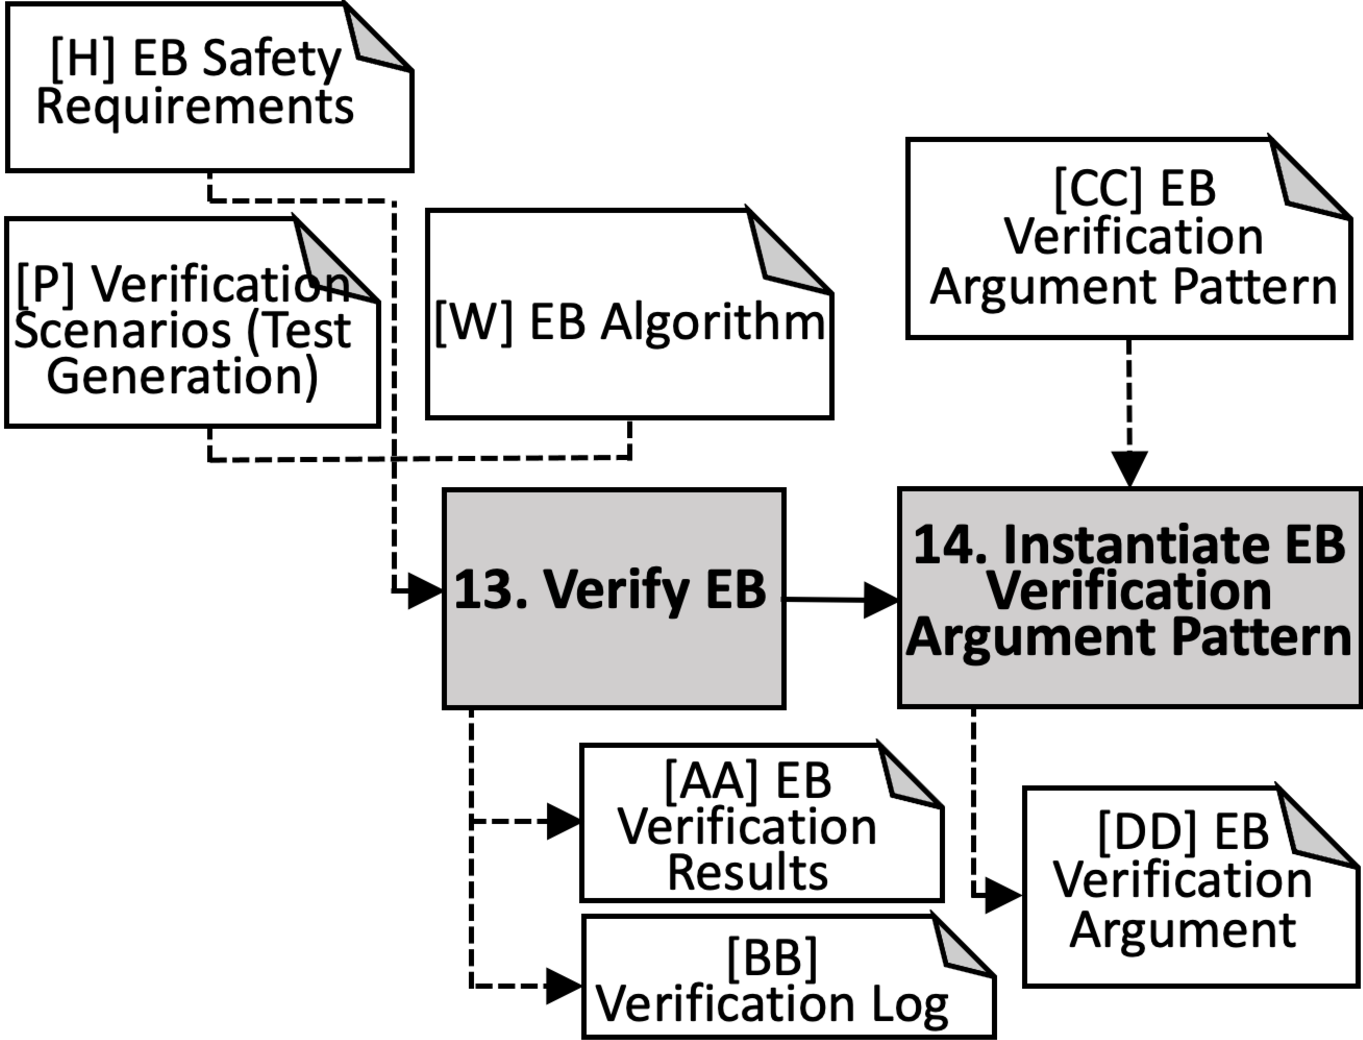
\includegraphics[width=0.9\textwidth]{figures/AERoS-Stage5.pdf}%AERoS-Stage5-v2.png    
			\vspace{-2ex}
			\caption{Stage 5: The AERoS verification process.}
			\label{amlas-a-stage5}
	      \end{minipage}%
      \hspace*{0.01\textwidth}
	\begin{minipage}[b]{.5\textwidth}
			\centering
			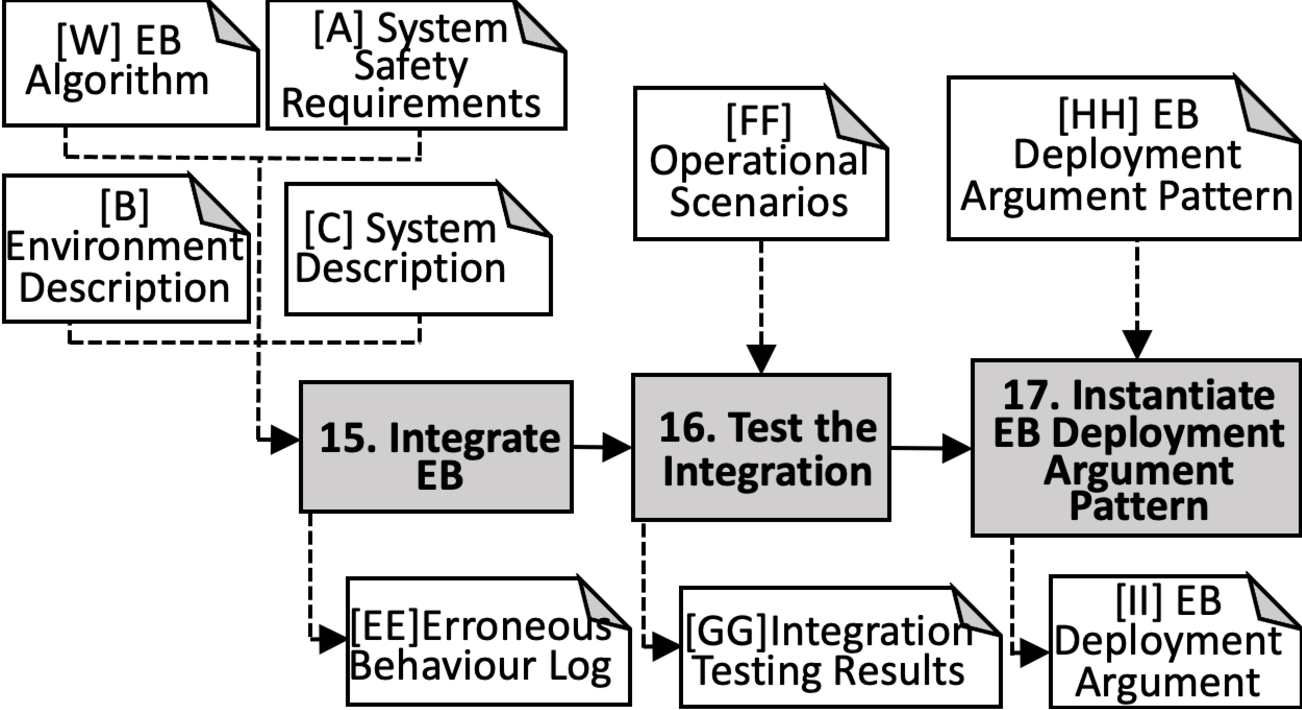
\includegraphics[width=0.99\textwidth]{figures/AERoS-Stage6.pdf}%AERoS-Stage6-v2.pn
			\vspace{-2ex}
			\caption{Stage 6: The AERoS model deployment assurance process.}
			\label{amlas-a-stage6}
		\end{minipage}
	\vspace{-4ex}
\end{figure}
%\begin{figure}[!t]
%	\centering
%	\begin{minipage}[b]{.47\textwidth}
%		\centering
%		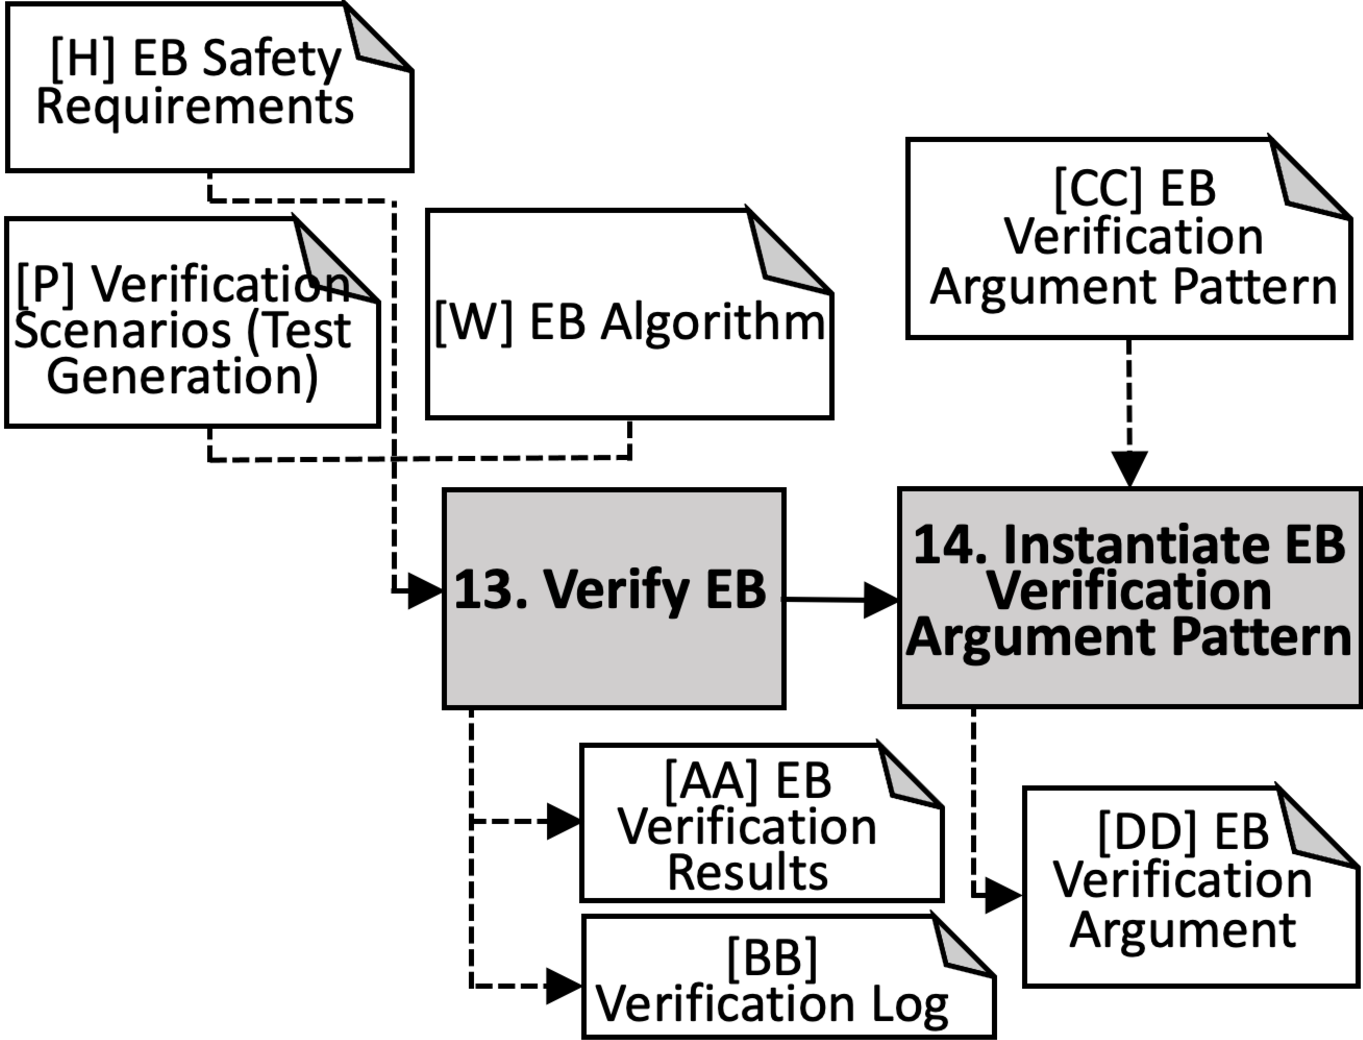
\includegraphics[width=0.9\textwidth]{figures/AERoS-Stage5.pdf}%AERoS-Stage5-v2.png    
%		\vspace{-2ex}
%		\caption{Stage 5: The AERoS verification process.}
%		\label{amlas-a-stage5}
%	\end{minipage}%
%	\hspace*{0.01\textwidth}
%	\begin{minipage}[b]{.5\textwidth}
%		\centering
%		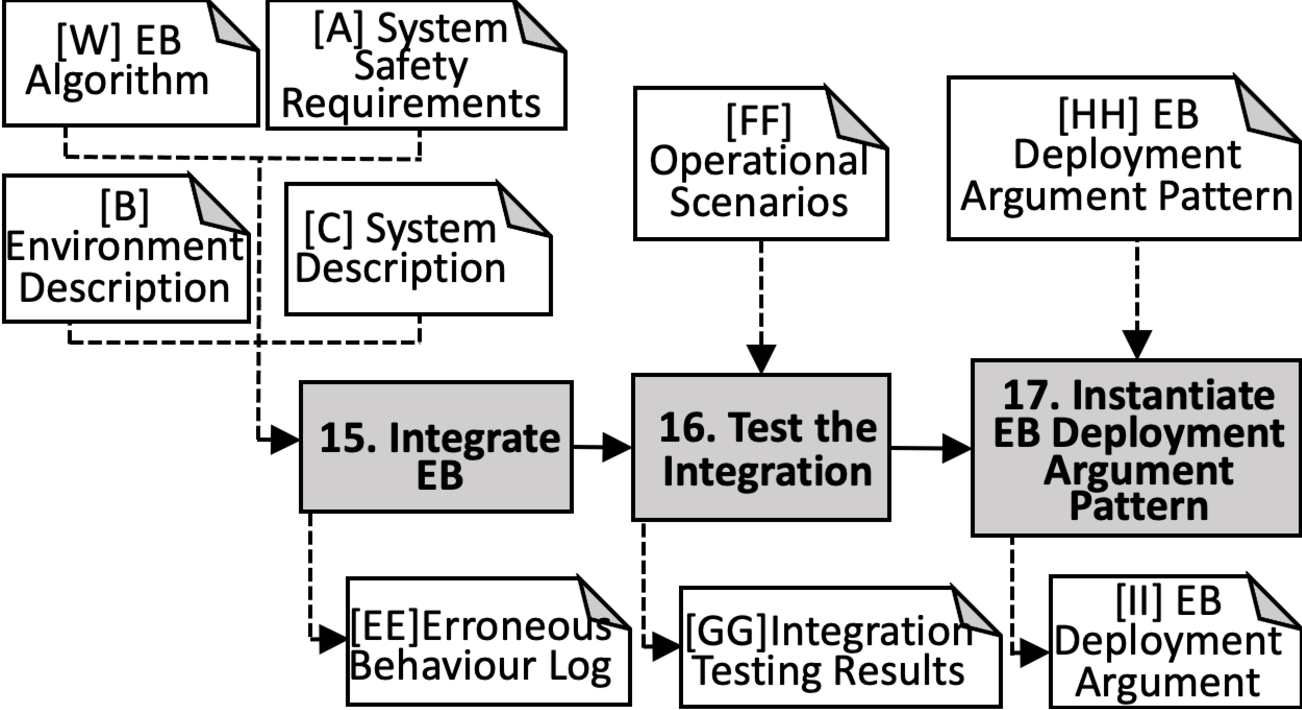
\includegraphics[width=0.99\textwidth]{figures/AERoS-Stage6.pdf}%AERoS-Stage6-v2.pn
%		\vspace{-2ex}
%		\caption{Stage 6: The AERoS model deployment assurance process.}
%		\label{amlas-a-stage6}
%	\end{minipage}
%	\vspace{-4ex}
%\end{figure}
%\noindent\textbf{Activity 15. Integrate EB} With the EB verified, the next step is to take the EB Algorithm [W], System Safety Requirements [A], Environment Description [B], and System Description [C] and integrate the EB with the system to be deployed (see Fig.~\ref{amlas-a-stage6}). 
\noindent\textbf{Activity 15. Integrate EB} With the EB verified, the next step is to take [W], [A], [B] and [C] as inputs, and integrate the EB with the system to be deployed (see Fig.~\ref{amlas-a-stage6}). In this activity, we use the inputs to this stage to inform the implementation of the EB and anticipate errors we might expect in the interactions between agents and the overall EB. Despite the rigorous validation and testing conducted in previous stages, there will still be a gap between the test environment and the intended, everyday-use, deployed scenario. The output, [EE] Erroneous Behaviour Log, captures these anticipated gaps between testing and reality and the differences in behaviour that may surface. 

\noindent\textbf{Activity 16. Test the Integration} Once the initial integration is complete, the physical implementation should undergo additional testing in which the system will be observed in multiple operational scenarios, as specified in [FF].

\emph{[FF] Operational Scenarios:} These scenarios should reflect the environment descriptions specified in [B], offering real-world situations to examine the behaviour of the integrated system. The testing of the integrated system in these true-to-operation environments should be conducted in a safe manner, ensuring that the entire multi-agent system can be shut down in an emergency. 
In the cloakroom, an example of [FF] may take the form of a deployment of agents in a controlled storage area that will not interfere with emergency services.
%
%\emph{[FF] Operational Scenarios:} These operational scenarios should reflect the environment descriptions specified in [B], offering real-world situations to examine the behaviour of the integrated system. The testing of the integrated system in these true-to-operation environments should be conducted in a safe manner and ensure that the entire multi-agent system can be shut down in an emergency. 
%In the cloakroom, an example of [FF] may take the form of a small deployment of agents in a controlled storage area that will not interfere with emergency services.
%
%In our use case, an example of [EE] may take the form of a small deployment of agents in a real but controlled storage area.\todo{More general, they should retire in an area/location that will not interfere with emergency services.}
%Ensuring that the entire multi-agent system can be shut down in an emergency, or providing shadow operators for groups of agents, taking over should the swarm behave erroneously. In our use case, an example of [EE] may take the form of a small deployment of agents in a real but controlled storage area.\todo{More general, they should retire in an area/location that will not interfere with emergency services.}

\emph{[GG] Integration Testing Results:} Results from the integration testing will be reported here, detailing how the system performs against the EB Safety Requirements [H] specified in Stage 2. 
The artefacts generated in this stage are used to instantiate the EB Deployment Argument Pattern [HH] in \textbf{Activity 17}.
\section{Conclusion} \label{discussion-conclusions}
%\todo{SW: Just an optional thought, but it feels like the discussion of the AERoS framework itself is missing. Could one of the tables be removed to make more space for discussion? I think a paragraph or two on advantages and limitations would be enough.}
Using AMLAS \cite{Hawkins2021} as a foundation, we proposed the six-stage development process AERoS. This process acts as guidance for those looking to construct swarm robot systems, particularly those that exhibit emergent behaviour through environmental and agent-to-agent interaction. The stages of AERoS break down the design of these systems to ensure that fundamental safety requirements are adhered to, even in instances of system degradation and compounded failures that should be expected, and managed, in robot swarms. We achieve this with an approach that allows for iteration of and feedback to the previous stages as issues of safety are encountered and investigated. We combine this iteration with repeated specification at each stage, observing the issue of safety through the lens of: data, modelling/behaviour design, verification, and deployment. 
% Added by Dhaminda to address Shane's comment
%While the iterative nature of AERoS is a key advantage, some limitations have been identified. 
%First, the scope of this work has been limited to investigating inherent swarm qualities and the emergent properties that arise from these. 
While the iterative nature of AERoS is a key advantage, the scope of this work has been limited to investigating inherent swarm qualities and the emergent properties that arise from these. 
However, one can expand on this, and consider adaptation of individual robots through techniques such as machine learning. % (e.g.\ by applying AMLAS).
%Second, we can broaden the evaluation by considering additional swarm use cases (e.g.\ monitoring fires in a natural environment, and also a social swarm), and by providing a worked example of the entire AERoS process.
Also, we can broaden the evaluation by considering additional swarm use cases (e.g.\ monitoring fires in a natural environment, and also a social swarm), and by providing a worked example of the entire AERoS process. 
While the focus of AERoS is to ensure the safety assurance of EB in swarms, the trustworthiness of an AS can be dependent on many factors other than safety, such as ethics, and governance and regulation, which we will investigate as part of future work.%the trustworthiness of an AS can be dependent on many other factors, such as ethics, and governance and regulation, which we will investigate as part of future work.
%While the focus of the AERoS process is to ensure the safety assurance of EB in swarms, the trustworthiness of an AS can be dependent on many factors other than safety, such as ethics, and governance and regulation, which we will investigate as part of future work.
%In future work, we intend to build on Porter et al.’s \cite{Porter2022} Principle-based Ethical Assurance Argument for AI and Autonomous Systems and develop ethics requirements for swarm robots around the ethical principles of beneficence, non-maleficence, respect for autonomy, and justice. 
%In addition to ethics requirements, we intend to introduce regulatory requirements into the consideration of AS specification. In particular, we observe the work of Macrae’s~\cite{macrae2021learning} Structural, Organisational, Technological, Epistemic, and Cultural (SOTEC) framework to help us identify sources of socio-technical risk in Autonomous and Intelligent systems. Viewing regulatory requirement analysis from a socio-technical perspective allows us to move away from a purely technical conception of requirements, and helps us design AS that better fit the organisation and operators’ work in which safety considerations are meaningful within the wider system and operational context. The relevance of SOTEC for crafting regulatory requirements for the swarms in the cloakroom as a safety assurance mechanism will be described in a future paper. 

%\subsubsection{Acknowledgements} Please place your acknowledgments at
%the end of the paper, preceded by an unnumbered run-in heading (i.e.
%3rd-level heading).

%\subsubsection*{Acknowledgments}
%\subsubsection{Acknowledgements} The authors would like to thank Alvin Wilby, John Downer, Jonathan Ives, and the AMLAS team for their fruitful comments. The work presented has been supported by the UKRI Trustworthy Autonomous Systems Node in Functionality under Grant EP/V026518/1. I.H.\ is supported by the Assuring Autonomy International Programme at the University of York.
%The work presented has been supported by the UK Engineering and Physical Sciences Research Council (EPSRC) under the grant [EP/V026518/1]. 
%
% ---- Bibliography ----
%
% BibTeX users should specify bibliography style 'splncs04'.
% References will then be sorted and formatted in the correct style.
%
\bibliographystyle{splncs04}
%\bibliography{AERoS-Bib}
\bibliography{AERoS-Bib-Shortened}
\vspace{-2ex}%\vspace{-2ex}
%
\end{document}
%%% Local Variables:
%%% mode: latex
%%% TeX-master: t
%%% End:
